% !TEX root = main.tex
%Specify document class
\documentclass[12pt,twoside,openany]{book}


%Packages to include
\usepackage[utf8]{inputenc}
\usepackage{setspace}

% \usepackage{mathpazo}
\usepackage{times}

% \usepackage[letterpaper,margin=1in,
% width=150mm,top=30mm,bottom=1in,
% bindingoffset=6mm]{geometry} % for book
\usepackage[letterpaper,margin=1in]{geometry} % for article
\usepackage{graphicx,wrapfig,lipsum}
\usepackage{bm}
\usepackage{indentfirst}
\usepackage{verbatim}
\usepackage{float}
\usepackage[shortlabels]{enumitem}
\usepackage{subcaption}
\usepackage{titlesec}
\usepackage[font={footnotesize}]{caption}
\usepackage{amsmath}
\usepackage{amssymb}


% \usepackage[subfigure,titles]{tocloft}


\usepackage{url}
\urlstyle{same}
\usepackage{xfrac}
\usepackage[backend=biber,style=phys,
	articletitle=true,biblabel=brackets,%
	chaptertitle=false,pageranges=false%
]{biblatex}
\addbibresource{references.bib}
% \DeclareFieldFormat[report]{title}{\printtext[doi/url-link]{\mkbibemph{#1}}}
\usepackage[nottoc,numbib]{tocbibind}
% \settocbibname{References}

\usepackage[table,xcdraw]{xcolor}
\usepackage{siunitx}

\usepackage[%
	colorlinks=true,
	pdfborder={0 0 0},
	linkcolor=blue,
	citecolor=blue,
	urlcolor=blue
]{hyperref}

%\bibliography{references.bib}
\usepackage[nameinlink]{cleveref}

%\linenumbers

%Set images folder
\graphicspath{ {Images/} }

%Set Header and Footer for all pages
\usepackage{fancyhdr}

\pagestyle{fancy}
\fancyhead{}
\fancyhead[LO]{\nouppercase{\textbf{\leftmark}}}
\fancyhead[RO,LE]{\textbf{\thepage}}
\fancyhead[RE]{\nouppercase{\textbf{\rightmark}}}
\fancyfoot{}
\renewcommand{\chaptermark}[1]{\markboth{#1}{}}


% To have the transparent command
\usepackage{svg}


\setlist[itemize]{topsep=\parskip}

%\setlength\abovecaptionskip{-5ex}
%\setlength{\textfloatsep}{0pt plus 1.0pt minus 2.0pt}
\setlength\belowcaptionskip{-3ex}

\usepackage[labelfont=bf]{caption}

%Eliminate extra page after title and table of contents
\let\cleardoublepage=\clearpage

%Make signature and date lines for title page
\newcommand*{\SignatureAndDate}[1]{
	\par\noindent\makebox[3.0in]{\hrulefill} \hfill\makebox[2.0in]{\hrulefill}
	\par\noindent\makebox[2.5in][l]{#1}      \hfill\makebox[2.0in][l]{Date}
}

%Main Body

\usepackage{lineno}
\makeatletter
\def\makeLineNumberLeft{%
	\linenumberfont\llap{\hb@xt@\linenumberwidth{\LineNumber\hss}\hskip\linenumbersep}% left line number
	\hskip\columnwidth% skip over a column of text
	\rlap{\hskip\linenumbersep\hb@xt@\linenumberwidth{\hss\LineNumber}}\hss}% right line number
\leftlinenumbers% Re-issue [left] option
\makeatother
\linenumbers


% Adding custom packages
% \usepackage{physics}

\begin{document}
% \pagenumbering{roman}
%Title Page
\begin{titlepage}
    \begin{center}
        \AddToHookNext{shipout/background}{\put(1in,-\textheight){\transparent{.1}
\includegraphics[width=\textwidth]{seal-rum-uprm-1280x1280px.png}}}

        %        \BgThispage
        % \vspace*{1cm}
      {\large
        \textbf{Trigger Studies for the Emerging Jets Analysis and Machine Learning for Tracker DQM at CMS Experiment}
       }

        \normalsize
        \vspace{0.55cm}
        by

        \vspace{0.55cm}

        \large
        Guillermo A. Fidalgo Rodríguez
        \vspace{1cm}

        A thesis presented for the degree of\\
        \vspace{0.5cm}
        MASTER OF SCIENCE \\
        % \vspace{0.5cm}
        in
        % \vspace{0.5cm}
        Physics\\
%        \vspace{0.5cm}
        UNIVERSITY OF PUERTO RICO\\
        MAYAGÜEZ CAMPUS\\
        2024
        \vspace{1.8cm}

        \end{center}

        Approved by:

        \vspace{2.0cm}

\SignatureAndDate{Sudhir Malik, Ph.D.}
\\President, Graduate Committee

\vspace{2.0cm}

\SignatureAndDate{Pablo Marrero, Ph.D.}
\\Member, Graduate Committee

\vspace{2.0cm}

\SignatureAndDate{Samuel Santana Col\'on, Ph.D.}
\\Member, Graduate Committee
\\Department Chairperson
% \vspace{1.0cm}

% \SignatureAndDate{Rafael A. Ramos, Ph.D.}
% \\Chairperson of the Department



\end{titlepage}


\frontmatter

\doublespace
\chapter{Abstract}

The Standard Model of Particle Physics (SM) has had a great track record over the decades. With the discovery of the top quark, the $\tau$ neutrino and the Higgs boson, the SM has proved it's effectiveness and prediction prowess. Yet, it leaves behind open questions regarding problems like Dark Matter and thus a need for new physics. This has brought up many exotic searches in hopes of answering the questions that the SM has yet to address.
To provide the necessary quality to search for new physics, physicists use the most complex machines ever designed.
The preponderance of cosmological evidence suggests that the density dark matter energy density of the Universe is around 5 times the amount of regular baryonic matter, and hence, experimental searches have been developed to explain this.
The CMS Collaboration has searched for signals of a dark matter model via the Emerging Jets analysis group.
As with all experiments in High Energy physics, acquiring high quality of data is paramount to achieve groundbreaking science. The CMS experiment achieves the collection of it's high quality data through the triggering and data acquisition systems put in place, but require manual labor to certify.
In this work I present trigger efficiency studies relevant to the Emerging Jets analysis. Moreover, I present my work
to improve the process of data certification in the DQM workflow implemented at the CMS Tracker DQM group. This work adds the automation of a new web application called the Machine Learning playground designed to improve DQM shifter efficiency in data certification.


% The Data Quality Monitoring (DQM) of CMS is a key asset to deliver high-quality data for physics analysis and it is used both in the online and offline environment. The current paradigm of the quality assessment is labor intensive and it is based on the scrutiny of a large number of histograms by detector experts comparing them with a reference. This project aims at applying recent progress in Machine Learning techniques to the automation of the DQM scrutiny. In particular the use of convolutional neural networks to spot problems in the acquired data is presented with particular attention to semi-supervised models (e.g. autoencoders) to define a classification strategy that doesn’t assume previous knowledge of failure modes. Real data from the hadron calorimeter of CMS are used to demonstrate the effectiveness of the proposed approach.

\vspace*{1cm}

\textit{Keywords}:  [Emerging Jets, Dark Matter, Quantum Chromodynamics, Machine Learning, Data Quality Monitoring]


\chapter{Resumen}

El Modelo Estándar de Física de Partículas (ME) ha tenido una historia existosa en las pasadas décadas. Con el descubrimiento del quark "cima", el neutrino $\tau$ y el bosón de Higgs, el ME ha mostrado su efectividad y su poder predictivo. Sin embargo, deja atrás preguntas abiertos con respecto a problemas como la Materia Oscura y por la tanto existe una necesidad de nueva física. Esto ha llevado a muchas búsquedas exóticas con la esperanza de responder a las preguntas que el Modelo Estándar aún no ha logrado responder. Para proporcionar la calidad necesaria para buscar nueva física, los físicos utilizan las máquinas más complejas que han sido diseñadas. La preponderancia de evidencia cosmológica sugiere que la densidad de energía de la materia oscura en el universo es aproximadamente 5 veces la densidad de materia bariónica regular. Por lo tanto se han desarrollado búsquedas experimentales para explicar esto. La Colaboración CMS ha buscado señales de un modelo de materia oscura a través del grupo de análisis de Jets Emergentes. Como en todos los experimentos en física de altas energías, adquirir datos de alta calidad es primordial para lograr ciencia innovadora.
El experimento CMS logra la recopilación de sus datos de alta calidad a través de los sistemas de ``trigger'' y adquisición de datos implementados pero requiere mucho trabajo manual para certificarlos. En este escrito, presento estudios de eficiencia de ``trigger'' relevantes para el análisis de Jets Emergentes. Además, presento mi trabajo para mejorar el proceso de la certificación de datos en el proceso de DQM implementado en el grupo de DQM del Tracker de CMS. Este trabajo añade la automatización de una nueva aplicación web llamada el ``Machine Learning Playground'', diseñada para mejorar la eficiencia de los trabajadores de turno de DQM en la certificación de datos.



\textit{Palabras claves}:  [Emerging Jets, Dark Matter, Quantum Chromodynamics, Machine Learning, Data Quality Monitoring]

\chapter*{Acknowledgments}

This work would not have been possible without the support of my family, colleagues, and friends. Firstly, I wish to thank my parents, family, and my partner Yarelis for their unwavering support. A special thanks to my advisor, Professor Sudhir Malik, who was fundamental to my academic growth, providing me with guidance and opportunities to shape me into what I am today. Thanks to Dr.~Scarlet Norberg (UPRM Post-Doc) for her continued support, guidance, and patience throughout this work. Scarlet also provided invaluable guidance even during my undergrad years at UPRM.

Thanks to the scientists and staff at the Fermilab LPC, in particular, Dr.~Gabriele Benelli for his phenomenal patience, leadership, and guidance throughout the years and during my visits at Fermilab. During the Emerging Jets analysis, I had a great professional opportunity to interact with scientists from the University of Maryland ( Dr. Sarah Eno, Dr. Long Wang, and Yi-Mu Chen), Fermilab (Dr. Kevin Pedro), and the University of Colorado Boulder (Dr. Kevin Stenson, Dr. Keith Ulmer, Dr. Alexx Perloff, Dr. Bill Ford, and Claire Savard) with special thanks to Dr.~Alexx Perloff for his guidance and mentoring.


I also wish to sincerely thank Fermilab LPC, the CMS Collaboration, CERN, and the Physics Department at the University of Puerto Rico at Mayagüez (UPRM) for providing me with facilities to conduct this research.
I would like to thank the National Science Foundation (NSF) for funding this work through the grant PHY-2111134 on "Physics Beyond Standard Model with the CMS Pixel Detector".

A lot of people have also contributed to my professional development which encompasses software training and broader impacts. A very special thanks to the NSF funded IRIS-HEP institute at Princeton University. While being a software training instructor at IRIS-HEP training programs I met several wonderful colleagues --  Kilian Lieret, Michel Villanueva, Wouter Deconick, Jim Pivarski, Henry Schreiner, Alexander Moreno -- who introduced me to state-of-the-art software in HEP.

I would also like to thank the Pathways to CU Physics Program and the University of Michigan - CERN REU program, respectively, for giving me a summer internship opportunity at CU Boulder and full semester scientific work at CERN.

This experience has provided me with several opportunities to disseminate my experience to high-school teachers and students in Puerto Rico and the international HEP community. Specifically, I would like to thank CROEM teacher Danelix Cordero who provided me initial opportunities for outreach work.

% A special thanks to all the wonderful people I have met in my early career as an aspiring physicist in HEP.
% Among these are those I met through the HEP Software Foundation (HSF) and IRIS-HEP whom have been influential for my professional and academic training in analysis software. In particular, Kilian Lieret, Michel Villanueva, Wouter Deconick, Jim Pivarski, Henry Schreiner, Alexander Moreno and many more that I cannot possibly fit into to these pages.


\singlespace
\tableofcontents
\listoffigures
\clearpage
\doublespace
\mainmatter

% \pagenumbering{arabic}
\chapter{Introduction}

The work for this thesis was performed with resources from European Organization for Nuclear Research (CERN)\footnote{\url{https://home.cern/about}}, the CMS Experiment\footnote{\url{http://cms.web.cern.ch/news/what-cms} or \url{https://cms.cern/detector}}, and the LHC Physics Center (LPC) at Fermi National Lab (FNAL).
CERN was founded in 1954 and is located at the Franco-Swiss border near Geneva. At CERN, physicists and engineers are probing the fundamental structure of the universe. They use the world's largest and most complex scientific instruments to study the basic constituents of matter --- the fundamental particles.
The instruments used at CERN are purpose-built particle accelerators and detectors. Accelerators boost beams of particles to high energies before the beams are made to collide with each other or with stationary targets. Detectors observe and record the results of these collisions. The accelerator at CERN is called the Large Hadron Collider (LHC), the largest machine ever built by humans and it collides particles (mostly protons) at just
$\qty[per-mode = symbol]{3}{\meter\per\second}$ under the speed of light.
The process gives physicists clues about how the particles interact and provides insights into the fundamental laws of nature. Nine\footnote{\url{https://home.cern/science/experiments}} experiments at the LHC use detectors to analyze particles produced by proton-proton collisions.
The biggest of these experiments, ATLAS and CMS, are general-purpose detectors designed to study the
fundamental nature of matter and fundamental forces and to look for new physics or evidence of particles that are beyond the Standard Model\footnote{\url{https://home.cern/about/physics/standard-model}}. Having two independently designed detectors is vital for cross-confirmation of any new discoveries made with minimal bias. The other two major detectors ALICE and LHCb, respectively, study a state of matter that was present just moments after the Big Bang and a preponderance of matter than antimatter.  Each experiment does important research that is key to understanding the universe that surrounds and makes us.
\Cref{ch:CMS} presents a basic description of the Large Hadron Collider and the CMS Detector.
\Cref{ch:emj} presents a description and background on the Emerging Jets theory and analysis.
\Cref{ch:HLT} develops the technical aspects and usage of the HLT system in CMS.
\Cref{ch:DQM} gives a brief description of what is Data Quality Monitoring (DQM) and its importance for CMS, as well as describe the Machine Learning tasks developed for it.
\Cref{ch:conclusion} summarizes the results of the analysis and ongoing DQM efforts.


\chapter{The CMS Detector\label{ch:CMS}}

CMS is one of the largest scientific collaborations in the history of mankind with over 4,000 participants from 42 countries and 182 institutions.
The CMS experiment is one of four detectors built at crossing sites of the LHC beams, and is one of two general purpose detectors (the other being the ATLAS detector) which have been designed to exploit the physics opportunities presented by the LHC.
It is designed to investigate various physical phenomena concerning the SM and beyond it, such as Supersymmetry, Extra Dimensions and Dark Matter.

The CMS detector essentially acts as a giant super highspeed camera that makes 3D images of the collisions that are produced at a rate of 40~\unit{MHz}.
As its name implies, the detector is a solenoid that is constructed around a superconducting magnet capable of producing a magnetic field of 3.8~\unit{\tesla}.
The magnetic coil is 13~\unit{m} long with an inner diameter of 6~\unit{m}, making it the largest superconducting magnet ever constructed.
The CMS detector itself  (as shown in \autoref{CMSLayout}) is over 28~\unit{m} long with a diameter of 15~\unit{m} and it has a weight of approximately 14,000~\unit{\tonne}.
Within the solenoid volume are a silicon pixel and strip tracker, a lead tungstate crystal electromagnetic calorimeter (ECAL), and a brass and scintillator hadron calorimeter (HCAL), each composed of a barrel and two endcap sections. Forward calorimeters extend the coverage of a coordinate known as the pseudorapidity ($\eta$) (see \Cref{fig:CMSCoord}) provided by the barrel and endcap detectors. Muons are measured in gas-ionization detectors embedded in the steel flux-return yoke outside the solenoid.

\begin{figure}
	\centering
	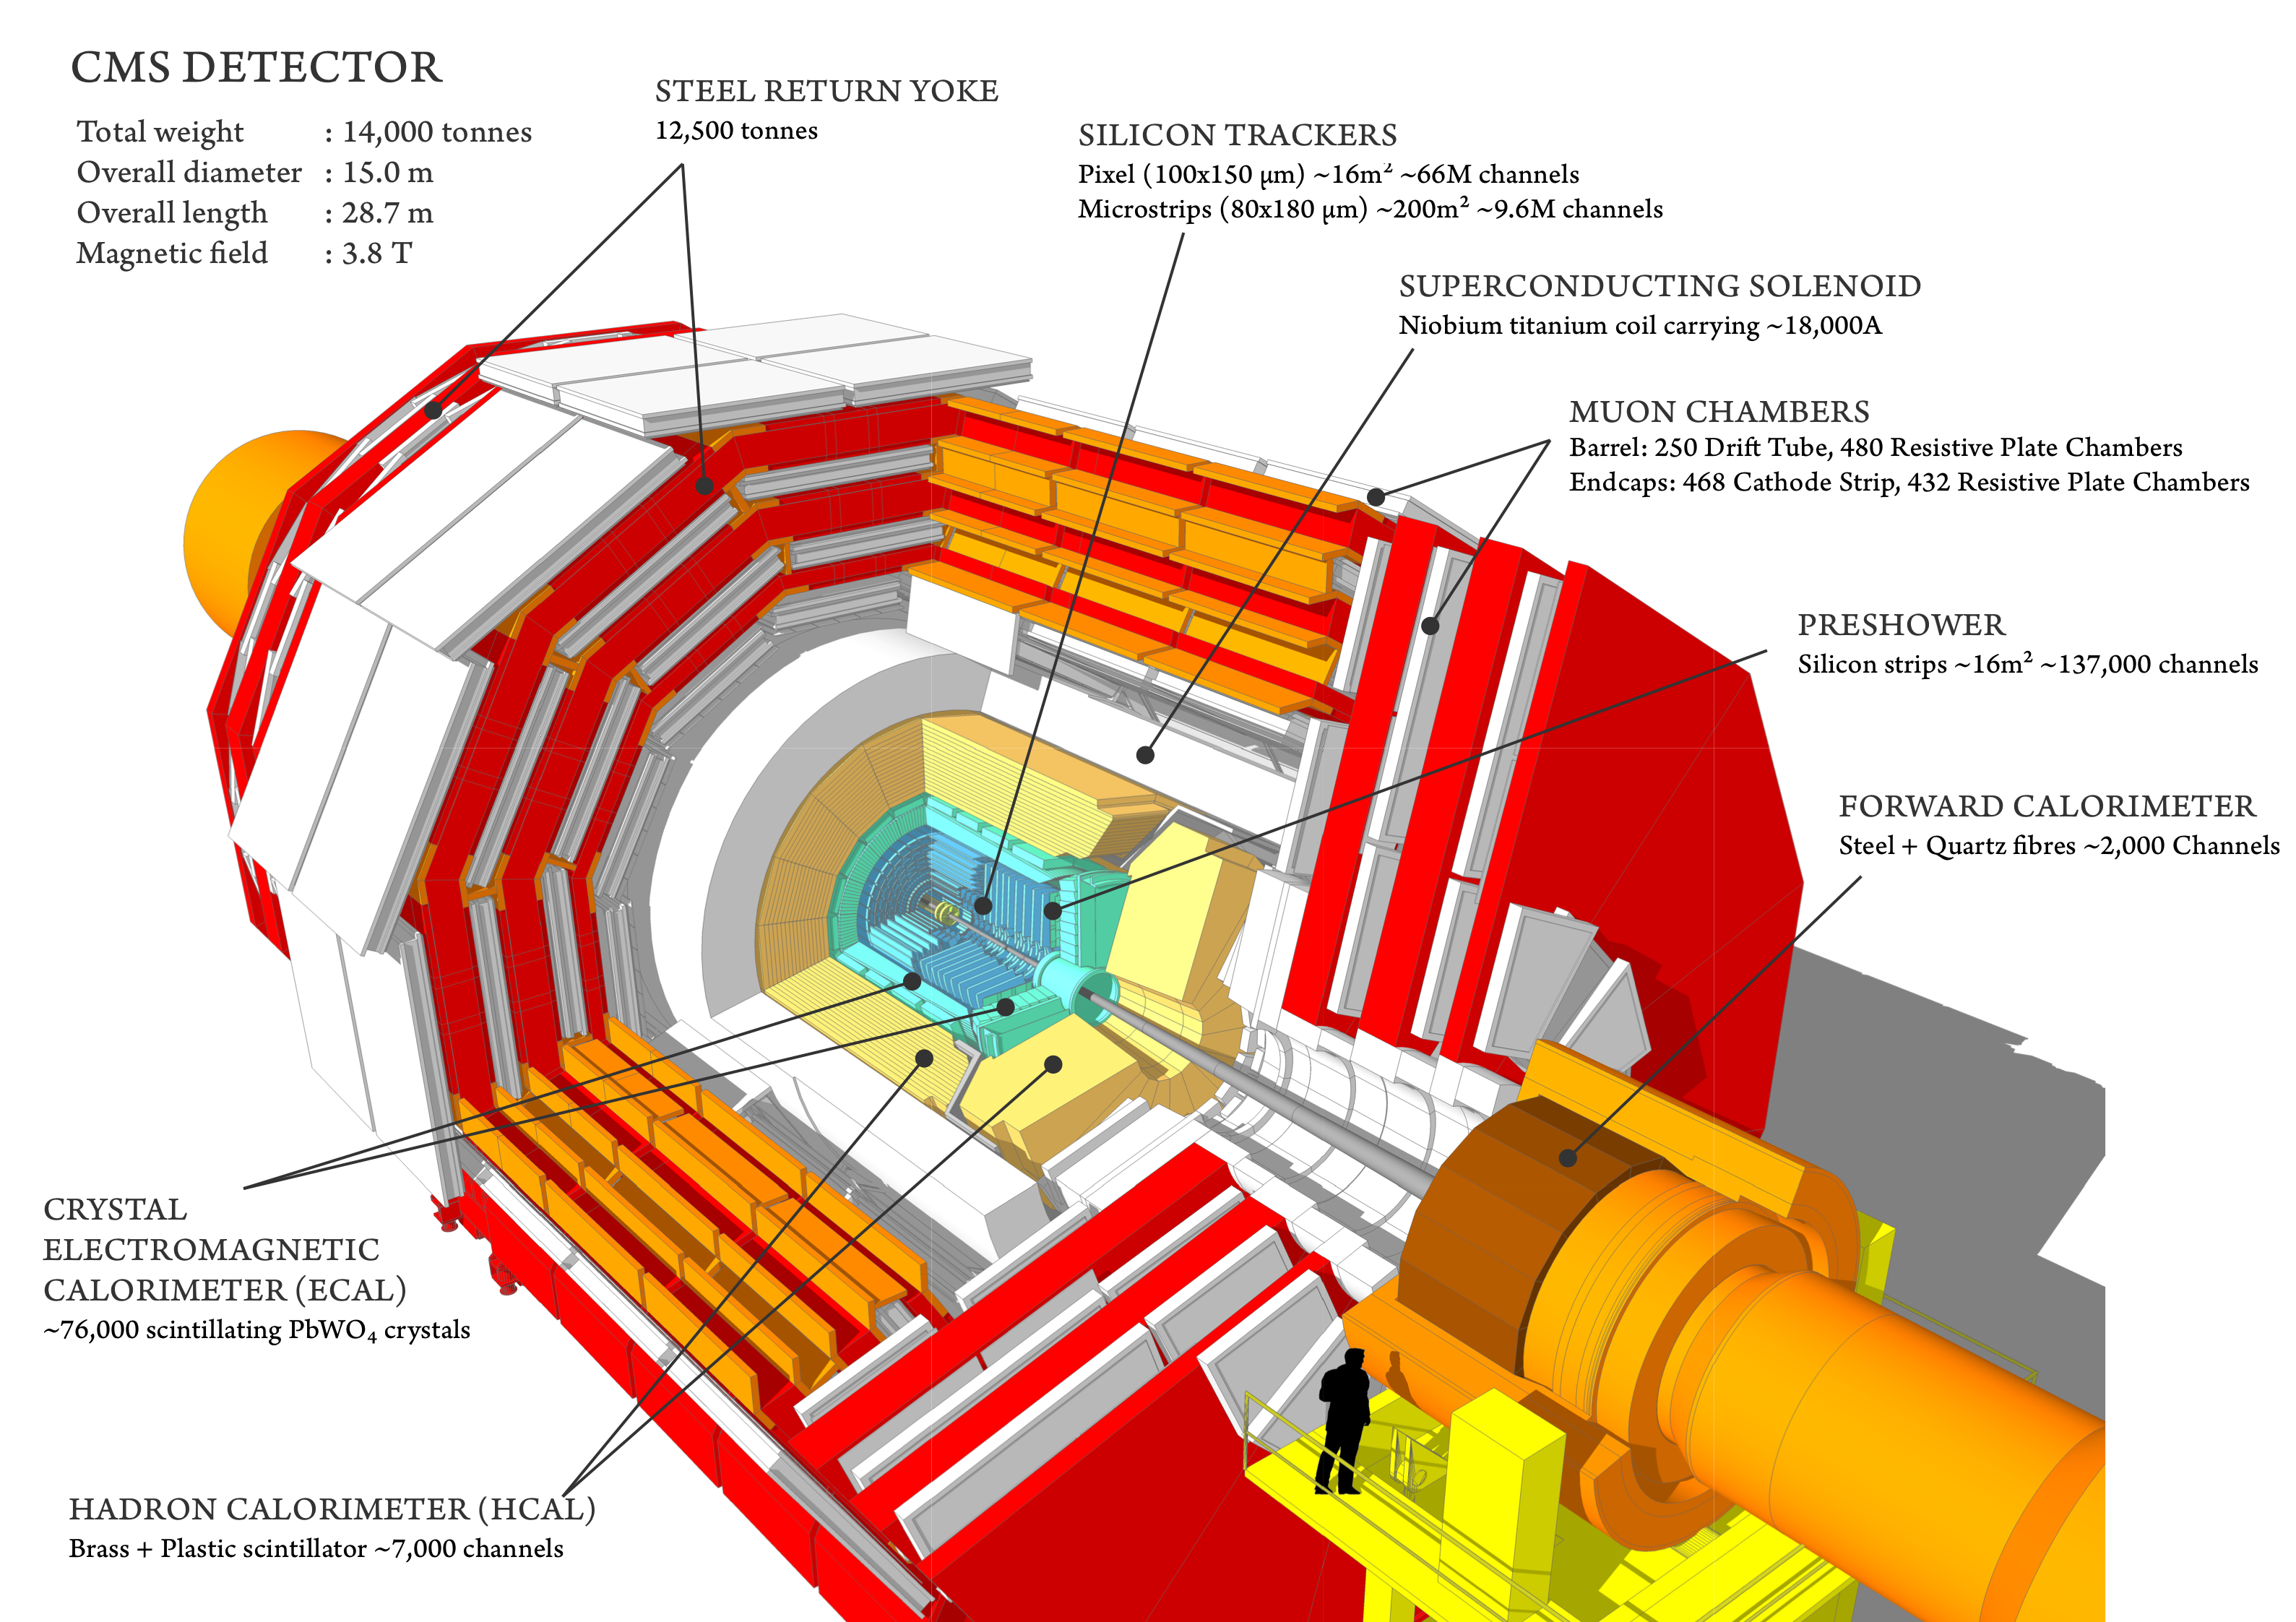
\includegraphics[width=\linewidth]{CMSLayout.png}
	\caption[CMS Detector]{The CMS Detector \cite{CMS_detector}}
	\label{CMSLayout}
\end{figure}
\begin{figure}
	\centering
	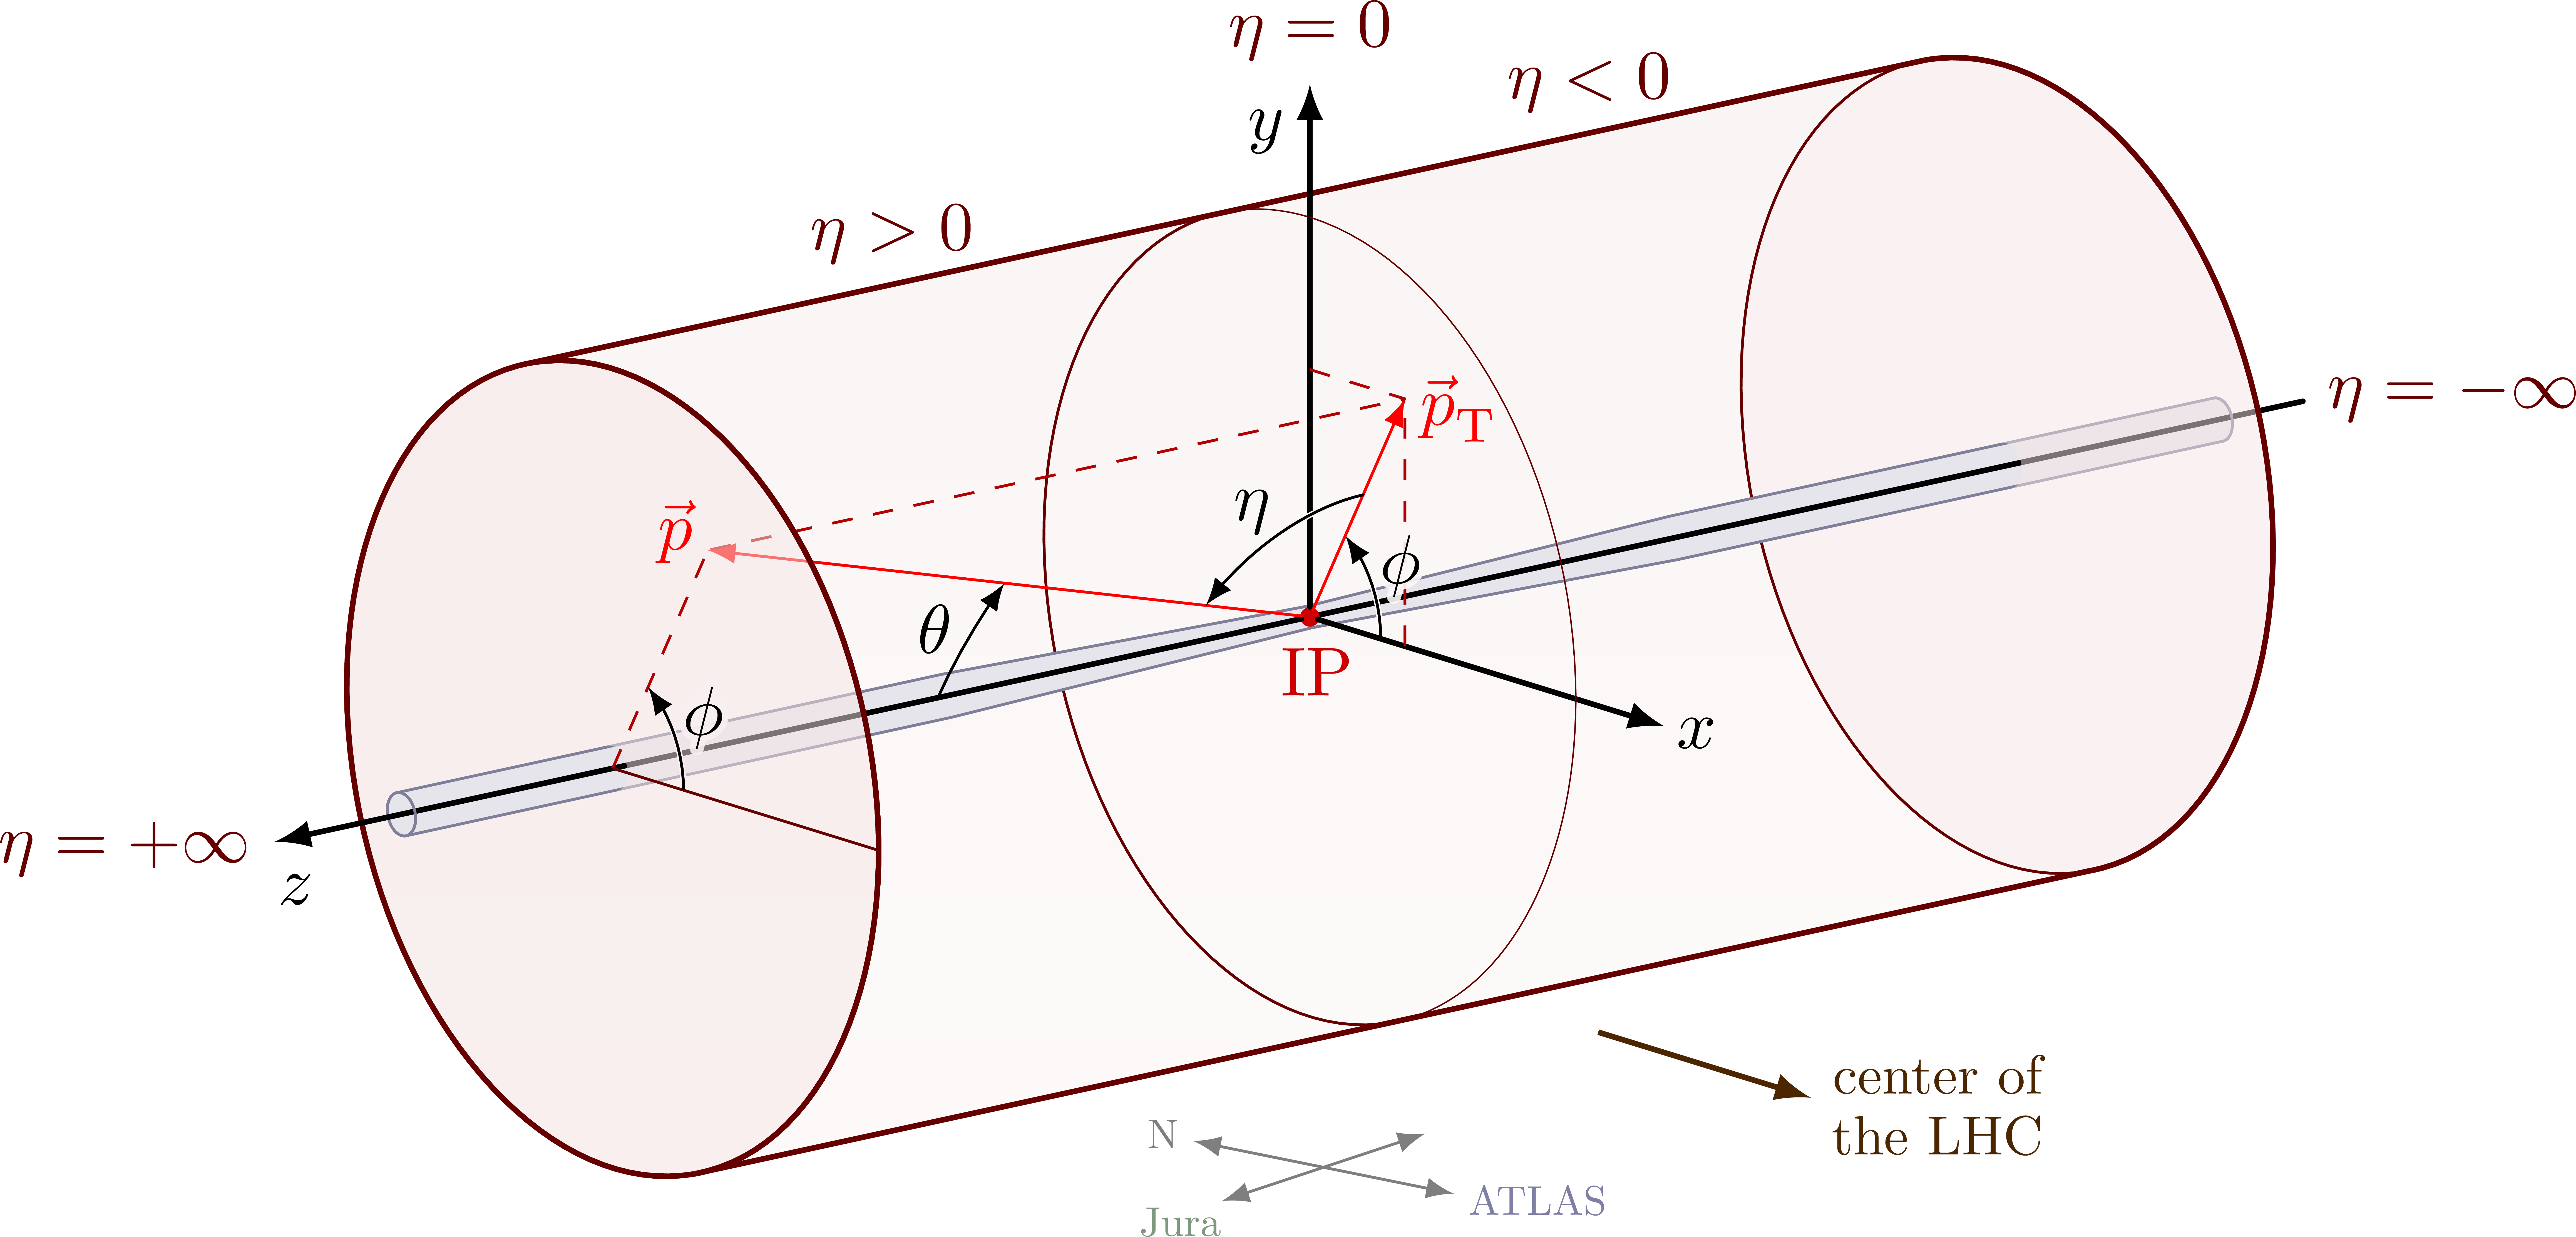
\includegraphics[width=.8\linewidth]{Images/CMS Coordinate.png}
	\caption[The CMS coordinate system]{The CMS coordinate system. From \cite{CMS_detector}}
	\label{fig:CMSCoord}
\end{figure}
The detector has an onion-like structure to capture all the particles that are produced in high-energy collisions.
A property of these particles that is exploited is their charge. Normally, particles produced in collisions travel in a straight line, but in the presence of a magnetic field, their paths are curved.
Except for the muon system, the rest of the sub-detectors lie inside the 3.8~\unit{T} magnetic field.
The Tracking devices are responsible for drawing the trajectory of the particles by using a computer program that reconstructs the path using electrical signals that are left by the particles as they move. The Calorimeters measure the energy of particles that pass through them by absorbing their energy with the intent of stopping them.
The particle identification detectors work by detecting radiation emitted by charged particles and using this information they can measure the speed, momentum, and mass of a particle. After the information is put together to make the “snapshot” of the collision one looks for results that do not fit the current theories or models in order to look for new physics.

\autoref{CMSLayers} depicts the particle detection process in CMS. Charged particles leave signatures in the inner tracking system, and the vertices from decaying short-lived particles can be identified. Photons, electrons, neutral pions and kaons are stopped in the crystals of the electromagnetic calorimeter (ECAL) and the scintillation light is used to determine the deposited energy. Hadrons punch through further and are generally stopped by the hadronic calorimeter (HCAL), where jets are confined and only the highest-energy hadrons and muons pass through the superconducting solenoid into the outer regions of the CMS barrel. Finally, muons are detected in the various muon detectors which interleave the return yoke of the magnet. Neutrinos escape from the CMS detector and are inferred from an imbalance of energy in the reconstructed event called missing transverse energy (MET or $\vec{p}_T^{\text{miss}}$).
More detailed descriptions of the CMS detector, together with a definition of the coordinate system used and the relevant kinematic variables, can be found in~\cite{CMS:2008xjf,CMS:2023gfb}.

\begin{figure}[h]
	\centering
	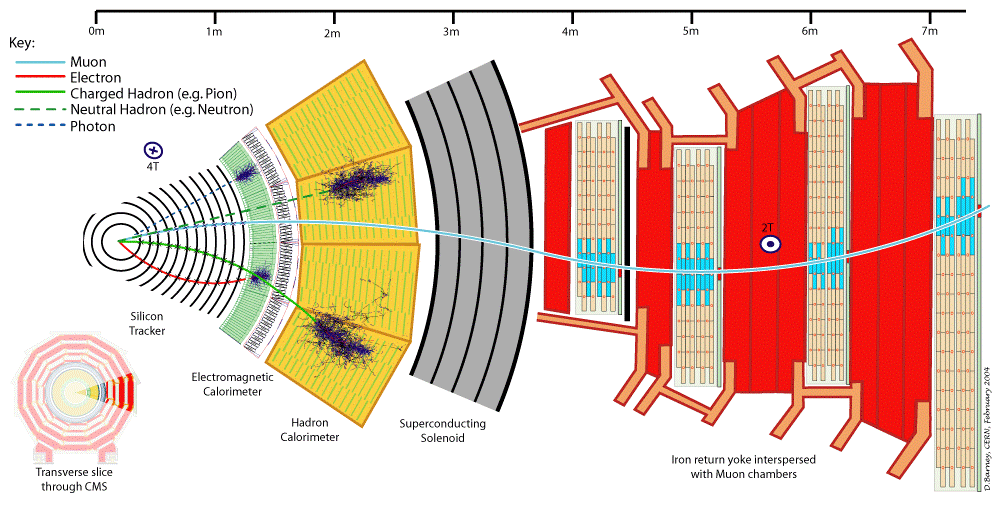
\includegraphics[width=.9\linewidth]{CMSLayers.png}
	\caption[Particle trajectories and footprint in CMS]{The trajectory of a particle traveling through the layers of the detector leaving behind it's signature footprint\label{CMSLayers}}
\end{figure}



% The project focusses specifically on data collected from one of the Calorimeters, - the Hadron Calorimeter (HCAL). The HCAL, as its name indicates, is designed to detect and measure the energy of hadrons or, particles that are composed of quarks and gluons, like protons and neutrons. Additionally, it provides an indirect measurement of the presence of non-interacting, uncharged particles such as neutrinos (missing energy) . Measuring these particles is important as they can tell us if new particles such as the Higgs boson or supersymmetric particles (much heavier versions of the standard particles we know) have been formed. The layers of the HCAL are structured in a staggered fashion to prevent any gaps that a particle might pass through undetected. There are two main parts: the barrel and the end caps. There are 36 barrel wedges that form the last layer of the detector inside the magnet coil, there is another layer outside this, and on the endcaps, there are another 36 wedges to detect particles that come out at shallow angles with respect to the beam line.


\chapter{Emerging Jets (EJs) \label{ch:emj}}


\section{Background information on EJs}

Many studies of dark matter require new physics that are beyond the Standard Model of Particle Physics (BSM) and searches with objects such as weakly interacting massive particles (WIMPs) have not been fruitful in this regard.
A class of models that includes electrically neutral fermions called “dark quarks” ($Q_{DK}$) that are not charged under the forces of SM but are charged under a new force in the dark sector (``dark QCD''), has properties similar to quantum chromodynamics (SM QCD).
These models naturally explain the observed mass densities of matter and dark matter.

The emerging jets concept arises from \cite{Schwaller:2015gea} where it was proposed to search for a new signature in the Run 1 dataset of the LHC Experiments and set limits on a combination of parameter ranges. The EJs model is a dark matter model that assumes that there is a QCD-like hidden sector. In particular, in these high-energy collisions, a heavy dark mediator ($X_{DK}$) is produced with a mass on the $\order{\text{TeV}}$, decaying into dark hadrons and mesons that further decay into SM particles.
Due to the hierarchy of GeV to TeV energy scales (see \cref{fig:dark-qcdmodel}), the decay process allows for dark matter particles to travel a measurable distance before decaying.
In \cref{fig:emj_production1} we see the production processes of the EJs signature. There are 2 ways of producing EJs in the LHC. First, is through gluon-gluon fusion and second is from quark anti-quark annihilation.
Both of these produce a pair of heavy dark mediators, each then decays into an SM quark (\textit{q}) and a dark quark (\Qdark).
Further on, we see from \cref{fig:full-chain} that the \Qdark will decay into \pidark.
Since these dark pions are unstable and do not carry a dark baryon number, they then decay after some measurable distance into SM particles\cite{Bai_2014} and form SM jets that we can detect.


\begin{figure}
	\centering
	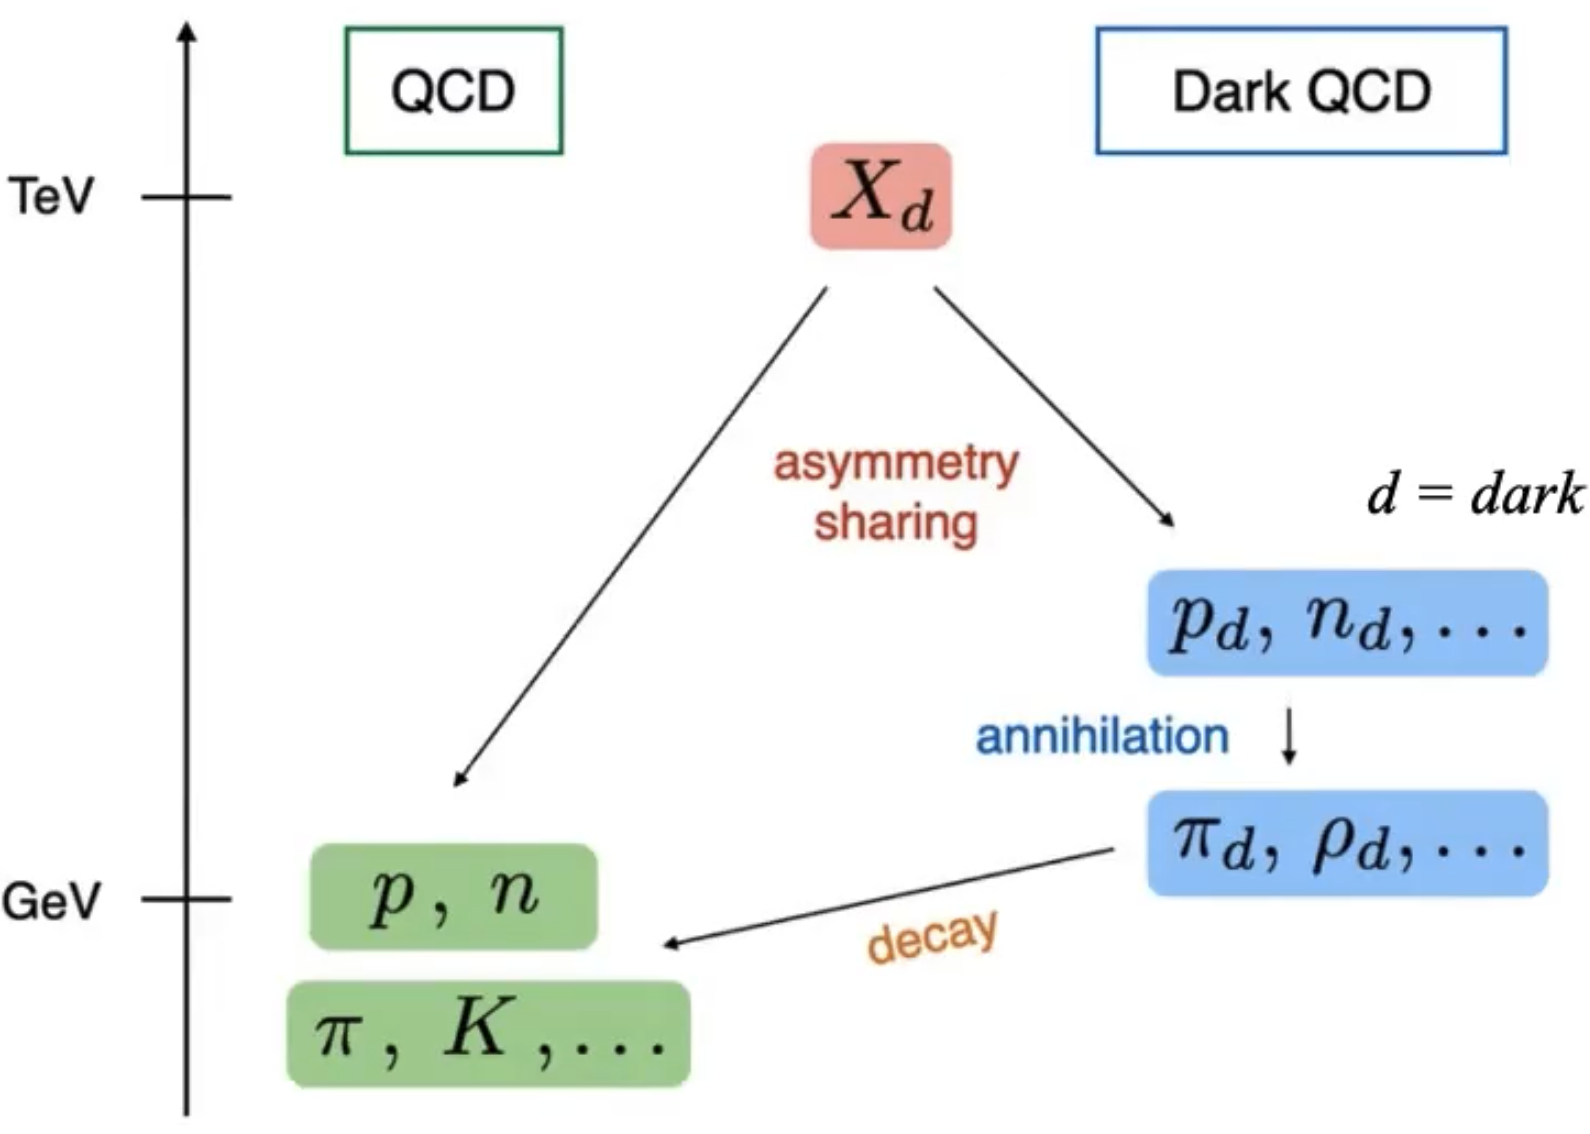
\includegraphics[width=0.8\linewidth]{Images/DarkQCDModel.png}
	\caption[The hierarchy of the GeV to TeV scales.]{The hierarchy of the GeV to TeV scales. In this model the dark scalar mediator $X_d$ couples to both dark and SM sectors. Reprinted from \cite{Schwaller:2015gea}}
	\label{fig:dark-qcdmodel}
\end{figure}


\begin{figure}
	\begin{center}
		\begin{subfigure}{.45\linewidth}
			\includegraphics*[width=\linewidth]{pdfs/BSSWPairProduction_ggFusion.pdf}
			\caption{gluon-gluon fusion}
		\end{subfigure}
		\begin{subfigure}{.45\linewidth}
			\includegraphics*[width=\linewidth]{pdfs/BSSWPairProduction_qqAnnihilation.pdf}
			\caption{quark anti-quark annihilation}
		\end{subfigure}
	\end{center}
	\caption[Emergin jets production modes]{Feynman diagrams for pair production of dark mediator particles, with mediators decay to an SM quark and a dark quark. The bar ($-$) over the quark symbols signify that they are anti-particles, as is the dagger ($\dagger$) over the \Mdark.}
	\label{fig:emj_production1}
\end{figure}

\begin{figure}
	\centering
	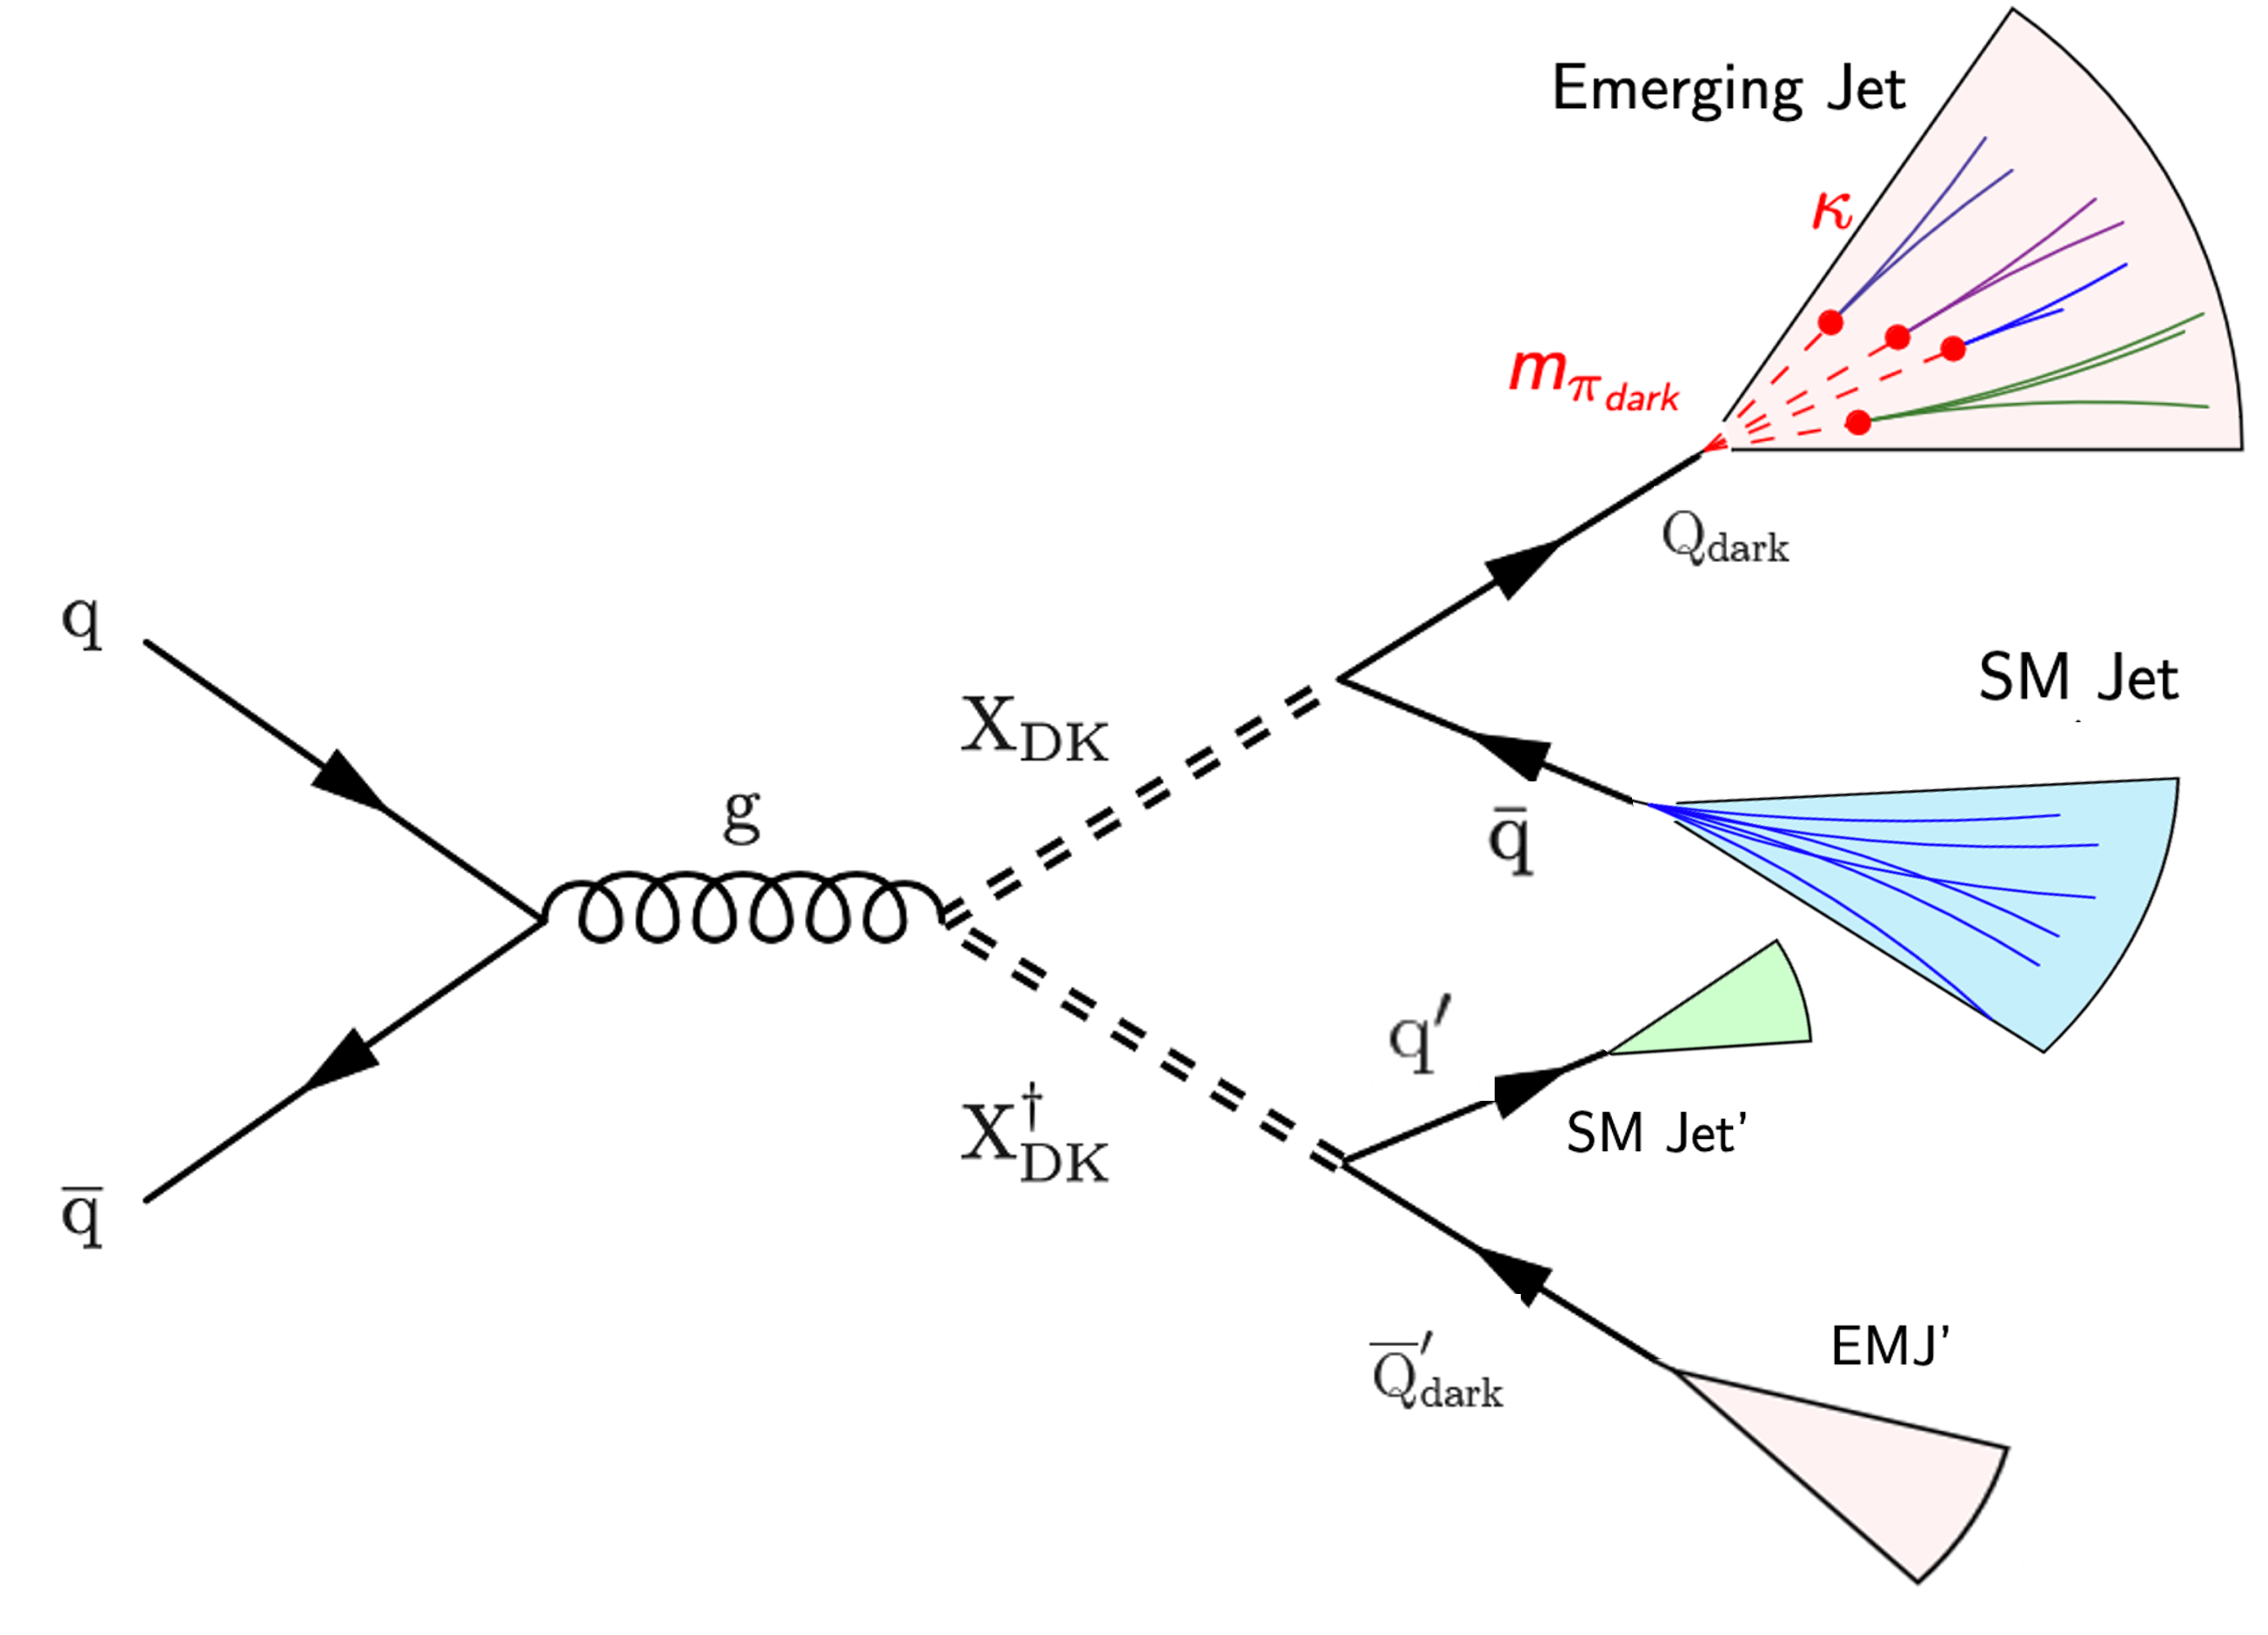
\includegraphics[width=.8\linewidth]{Images/EMJ_production.png}
	\caption{Example of the full chain of one production mode.}
	\label{fig:full-chain}
\end{figure}

\begin{figure}
	\centering
	\begin{subfigure}{.45\linewidth}
		\includegraphics*[width=\textwidth]{pdfs/FlavoredSchematicOfEvent.pdf}
		\caption{Flavor aligned}
		\label{fig:emj_prod2A}
	\end{subfigure}
	\begin{subfigure}{.45\linewidth}
		\includegraphics*[width=\textwidth]{pdfs/UnflavoredSchematicOfEvent.pdf}
		\caption{Unflavored}
	\end{subfigure}
	\caption[Shorter version of the production modes for the Emerging Jets models.]{Shorter version of the production modes for the Emerging Jets models. On the left, we show the flavor-aligned model where all \Qdark couple to down-type SM quarks only (d,s,b).
		This model has \pidark variable lifetimes (\ctaudpi ) which depend on their composition and the Yukawa coupling constant ($\kappa$) between the mediator particle, the dark quarks, and the SM down quark. This parameter represents the lifetime of each track inside emerging jets.
		On the right, we show the simpler unflavored model. This produces \Qdark that couple to the down-quark only and all \pidark lifetimes are the same.}
	\label{fig:emj_production2}
\end{figure}


% Add explanation on two EMJ models
In the experimental searches \cite{sirunyan2019search,CMS:2024gxp} the TeV scale has been explored searching for the EJs signature.
The full Run 2 dataset is used in the latest search for emerging jets using the data collected by the CMS Collaboration in 2016--2018 using pp collisions at a center-of-mass energy of 13 TeV accumulating 138\unit{\per\femto\barn} worth of data\cite{CMS:2024gxp}.
In the latest search, we studied the models described in \cite{Bai_2014,Schwaller:2015gea,Renner_2018} in which we expanded on the phase space searched in \cite{sirunyan2019search} and included the second model portrayed in \cref{fig:emj_prod2A} that allows for the \Qdark to couple to all down-type quarks. In this model, each dark subcomponent (or \pidark) within the dark jet can subsequently decay into standard model particles at different distances along the jet axis.
Here, lifetimes for the dark mesons are dependent on the \Qdark composition and the Yukawa coupling constant ($\kappa$) between the dark quarks and the SM down quark.
In the unflavored model, all \Qdark are degenerate, while in the flavored model, three dark quark flavors with non-degenerate couplings are considered.
For the unflavored model, the average decay length of a dark pion is given by \cref{eq:unflavored-ctau}
\begin{equation}
	\ctaudpi = 80~\unit{mm} \pgroup{\frac{1}{\kappa^4}} \pgroup{\frac{2 ~\unit{GeV} }{f_{\pidark}}}^2 \pgroup{\frac{100 ~\unit{MeV}}{m_\text{d}} }^2 \pgroup{\frac{2~\unit{GeV}}{m_{\pidark}}} \pgroup{\frac{m_{\Mdark}}{1~\unit{TeV}}}^4
	\label{eq:unflavored-ctau}
\end{equation}
where $f_{\pidark}$ is the dark pion decay constant, $m_\text{d}$ is the mass of the SM down quark, and $m_{\pidark}$ is the dark pion mass. In the flavored aligned model, the coupling constant is now a matrix $\kappa_{\alpha i}$ where the subscript $\alpha ~(i)$ denotes flavors of dark (SM) quarks. In this case, the average decay length for dark mesons is given by \cref{eq:flavored-ctau}
\begin{equation}
	\small
	\ctaudpi^{\alpha \beta} = \dfrac{8\pi m^4_{\Mdark}}{ N_c m_{\pidark} f^2_{\pidark} \displaystyle \sum_{i,j} \abs{\kappa_{\alpha i} \kappa_{\beta j}^*}^2 \pgroup{m_i^2 + m_j^2} \sqrt{ \pgroup{1- \dfrac{(m_i^2 + m_j^2)^2 }{m^2_{\pidark}} } \pgroup{1- \dfrac{(m_i^2 - m_j^2)^2 }{m^2_{\pidark}} } } }
	\label{eq:flavored-ctau}
\end{equation}
where $m_{\Mdark}$ is the mediator mass, $N_c$ is the SM color factor and $m_i, m_j$ are the masses of the SM quarks with flavor indices $i, j$, respectively\cite{CMS:2024gxp}.
\Cref{fig:lifetimes} shows the different $c\tau$ for a given $m_{\pidark}$ based on the \pidark composition in the flavor-aligned model. In general, the lifetime of the dark pions goes down as their mass increases, as opposed to the unflavored model where the lifetimes are the same for all \pidark.
\begin{figure}[b]
	\centering
	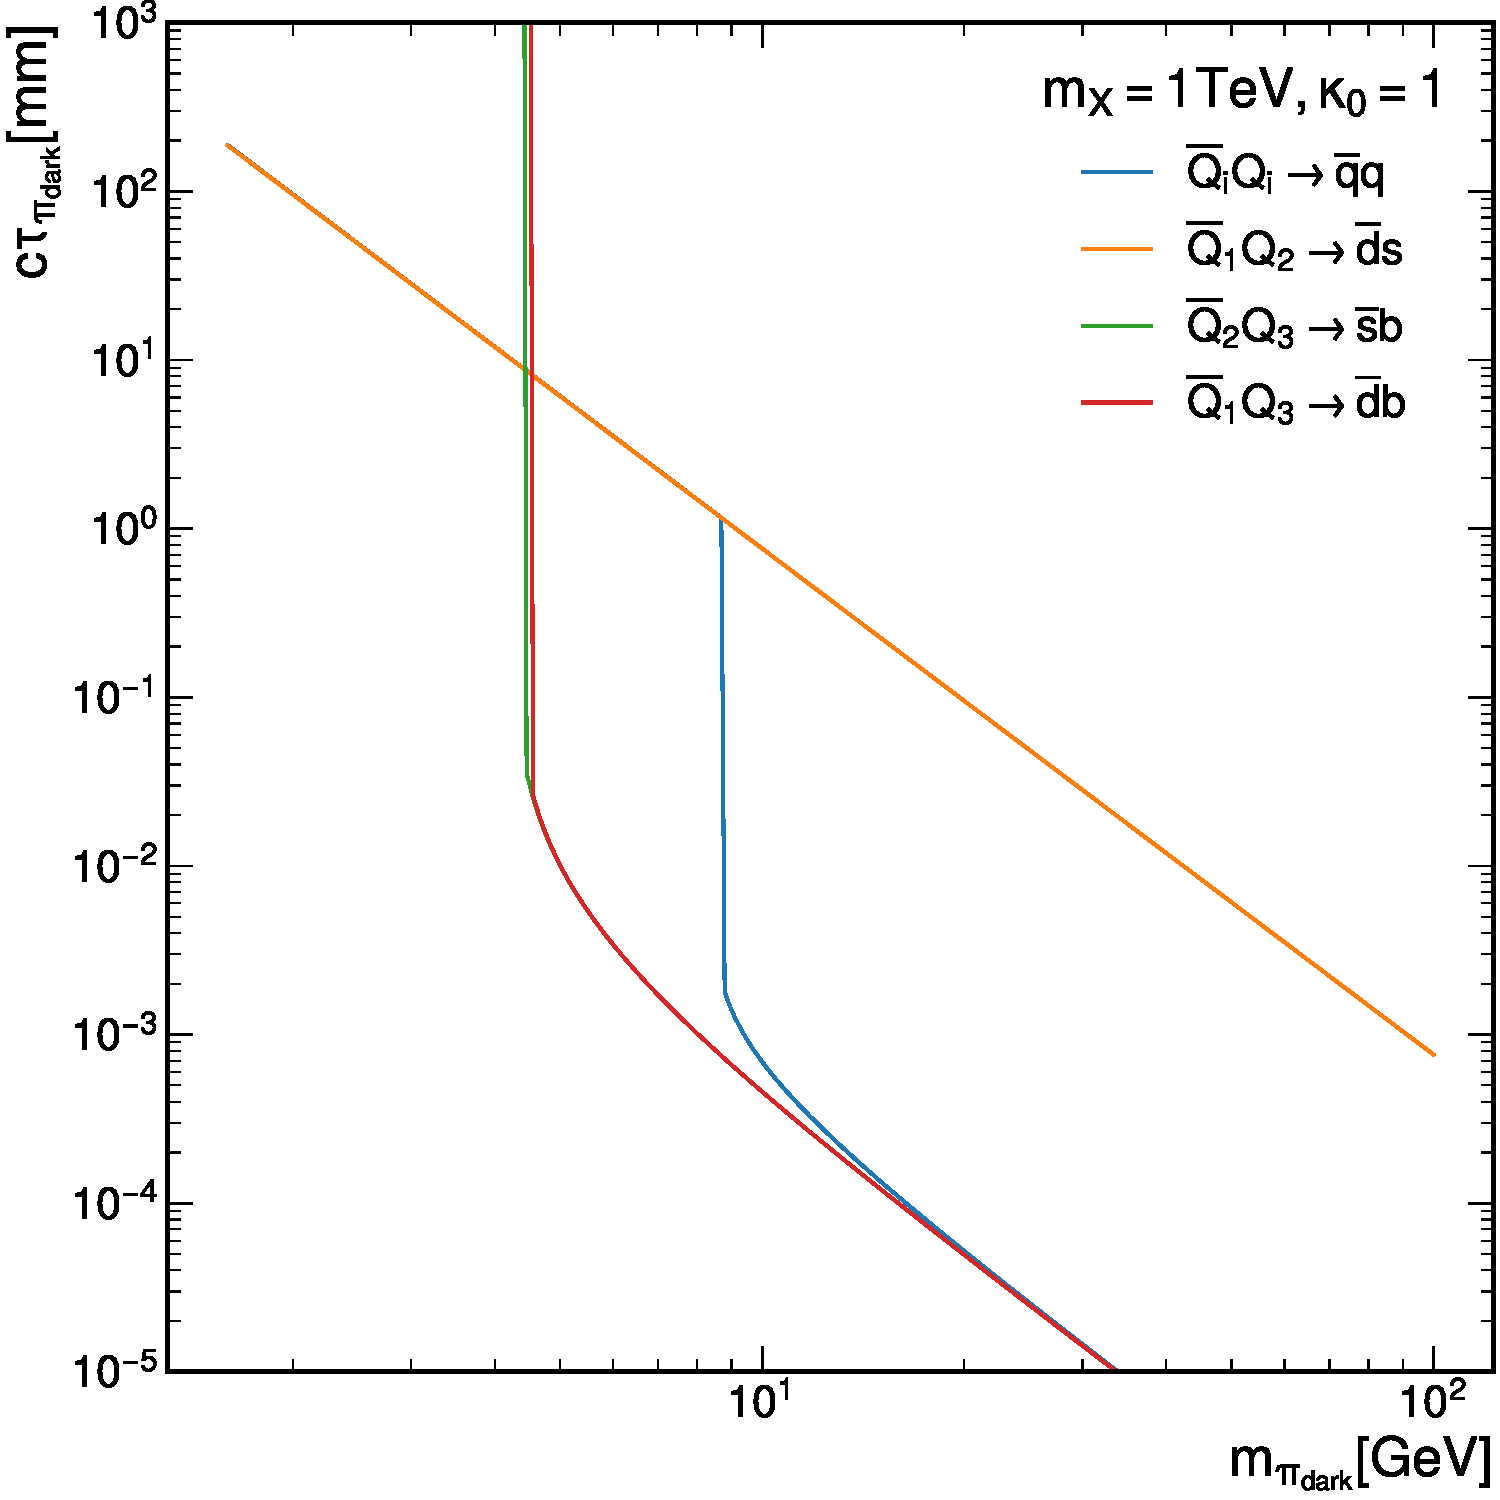
\includegraphics[width=.65\linewidth]{Images/pdfs/FlavoredLifetime.pdf}
	\caption[Lifetimes of the dark pions as a function of their mass.]{Lifetime of the \pidark as a function of the $m_{\pidark}$ in the flavor-aligned model. The jumps in the plot are indications of new energy states becoming available.}
	\label{fig:lifetimes}
\end{figure}

This latest search makes use of the increased amount of data, and the introduction of machine learning techniques to search for emerging jets.
We can see from \cref{fig:decay-distance} that this model has some distribution of the decay lengths in the order $\order{\unit{mm} - \unit{m}}$. The CMS detector is hence, sensitive to this phenomenon.
\Cref{fig:2emj_inCMS} illustrates how two EJs would look in a detector. It is assumed that from the high-energy collisions, dark quarks with enough energy hadronize and decay into dark mesons like pions ($\pi_{Dk}$). In the detector the SM quarks hadronize to produce SM jets and the dark quarks would also hadronize to make dark jets. The main signature for the analysis is to look for events that have high event energy, in particular in the form of a quantity known as $H_T$. The $H_T$ of an event is defined as the scalar sum of the transverse momentum ($\Vec{p}_T$) of the 4 leading jets (2 EJs, 2 SM jets).
\begin{equation}
	H_T = \sum_{i=1}^4 p_T^i
\end{equation}

\begin{figure}[tb]
	\centering
	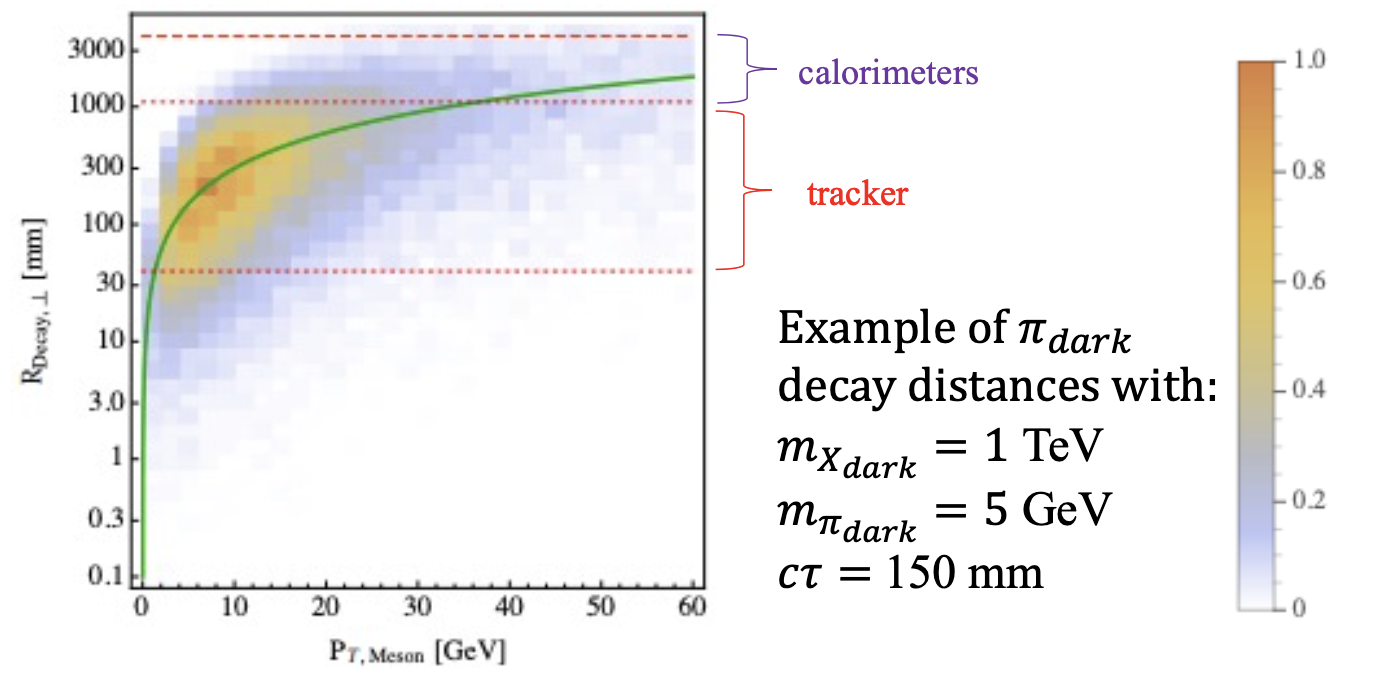
\includegraphics[width=.75\linewidth]{Images/Decay-distances-emj.png}
	\caption[2D distributions of decay distances and $\pi_{DK}$ momentum]{2D distribution between the decay distances and the $\pi_{DK}$ momentum. Reprinted from \cite{Schwaller:2015gea}}
	\label{fig:decay-distance}
\end{figure}

The free parameter ranges that are studied are:
\begin{itemize}
	\item $m_{\Mdark} \in [1,2.5]$ TeV
	\item $m_{\pidark} \leq 20$ GeV
	\item $\ctaudpi \leq 500$ mm
\end{itemize}


\begin{figure}
	\centering
	\includegraphics[width=.58\linewidth]{emj_detector.png}
	\caption[Illustration of the emerging jets forming in a detector]{An illustration of the pair production of dark quarks forming two emerging jets. Dashed lines represent the dark mesons as they do not interact with the detector. After traveling some distance, each dark pion decays into Standard Model particles, creating a small jet represented by solid colored lines. Because of the exponential decay, each set of SM particles originates at a different distance from the interaction point, so the jet slowly emerges into the detector. Figure and description adapted from \cite{Schwaller:2015gea}}
	\label{fig:2emj_inCMS}
\end{figure}


\clearpage

\section{Trigger Efficiency and Scale Factor studies}


With a beam spacing of 25\unit{ns}, beam crossings occur in the CMS detector at a rate of 40 million per second 40\unit{\MHz}.
An additional complication is the approximately $>$25 interactions (``pileup'') that occur with each beam crossing -- thus giving 1 billion events occurring in the CMS detector every second. To extract physics from these interactions it is vital to have fast electronics and good resolution (proton-proton interactions are very messy and produce hundreds or thousands of particle candidates) and, because these events occur far too quickly to all be recorded and would take up vast amounts of disk space to store what are, for the majority, uninteresting events, very precise ``triggering'' is required.

Events of interest are selected using a two-tiered trigger system. The first level (L1), composed of custom hardware processors, uses information from the calorimeters and muon detectors to select events at a rate of around 100~\unit{kHz} within a fixed latency of 4~\unit{\us} \cite{CMS:2020cmk}. The second level, known as the high-level trigger (HLT), consists of a farm of processors running a version of the full event reconstruction software optimized for fast processing and reduces the event rate to around 1\unit{kHz} before data storage~\cite{CMS:2016ngn}.

There are multiple types of triggers, and each will determine the kind of physics dataset that the data will be classified under. There are a few main datasets used to classify physics data, the ones relevant to the analysis are \emph{JetHT} for 2016-2018 and \emph{SinglePhoton}/\emph{EGamma} for 2016-2017/2018. These are considered to be orthogonal datasets as we do not expect a large overlap of the physics process that take place in them. Each category\footnote{also called a data stream} is comprised of an exhaustive list of ``trigger paths'' that are executed to decide what more specific conditions or subprocesses have taken place to record the events.
The $H_T$ triggers chosen are the triggers with the lowest online $H_T$ threshold that are not pre-scaled. The configurations used for this analysis for the \textit{JetHT} data stream are:

\begin{itemize}
	\item \verb|HLT_PFHT900_v* OR HLT_PFJet450_v*| for 2016. The addition of a jet trigger path in an OR configuration is the recommended path to mitigate an observed inefficiency at high values of $H_T$ caused by the Level-1 trigger firmware issues for 2016.
	\item \verb|HLT_PFHT1050_v*| for 2017 and 2018.
\end{itemize}

The paths used for the \textit{SinglePhoton} data stream are:
\begin{itemize}
	\item \verb|Photon165_HE10_v*| for 2016/2016 HIPM
	\item \verb|Photon200_v*| for 2017/2018
\end{itemize}

We also have a simulation equivalent of these main datasets where we have access to the ground truth (Generator-Level) information of the simulated events, called Monte Carlo (MC) simulations.
Though not directly used to draw the conclusions of the search, SM MC samples are used to develop the analysis strategy. The SM multi-jet MC samples are used as a stand-in for expected background events in the \textit{JetHT} data and are used for event/object selection optimization, closure tests and evaluation of uncertainties. The $\gamma$+jets MC samples are used as a stand-in for the \textit{SinglePhoton} data stream, used for template histogram generation, and are compared with the multi-jet MC to evaluate uncertainties associated with \textit{JetHT}/\textit{SinglePhoton} environment differences\cite{CMS:2024gxp}.


The calculation of the trigger efficiency is carried out by using the orthogonal \verb|HLT_Mu50_v*| trigger as the reference trigger. The offline $H_T$ threshold at which the trigger can be considered to be fully efficient was estimated by fitting the trigger efficiency as a function of $H_T$ to an error function (erf) and an algebraic function ($f$):

\begin{align}
	\text{erf}(H_T ;\ A,B,C) & = \frac A2 \left[1+ \text{erf}\left(\dfrac{H_T - |B|}{C}\right) \right]\label{eq:erf} \\
	f(H_T ;\ A,B,C,D)        & = A \dfrac{\frac{H_T - B}{C}}{1+ \left(\frac{H_T - B}{C}\right)^2} + D \label{eq:alg}
\end{align}

Where \cref{eq:erf,eq:alg} are modeled after the sigmoid-like functions
\[
	\text{erf}(x) = \frac{2}{\sqrt{\pi}} \int_0^x e^{-t^2} \dd{t}
\]
\[
	f(x)=\frac{x}{1+x^{2}}
\]


The fit result is used to determine the threshold at which the $H_T$ trigger is expected to reach 99\% of their plateau value. This is also to assist in the termination of the offline $H_T$ cut applied to signal event selection, to make sure that signal events are not impacted too much by the trigger turn-on effects. \Cref{fig:HT_efficiencies} shows the trigger efficiency as a function of event $H_T$ evaluated in the 4 data collection eras using the \textit{JetHT} data stream compared with QCD simulation along with an estimate of the trigger plateau value.
More specifically, \cref{fig:HT_eff_16,fig:HT_eff_16_HIPM,fig:HT_eff_17,fig:HT_eff_18} compare efficiency for \HT trigger as a function of event \HT measured relative to \verb|HLT_Mu50_v*| in data (black) and QCD MC (gray) and fit the algebraic function \textit{f} (line). With the computation of the efficiency at each range of \HT, we can compute the ratio between the \HT in data and MC. The ratio of the trigger efficiency in data vs. that in QCD MC is applied to each signal MC event as an $H_T$-dependent scaling factor, and the difference in the event acceptance of applying the scale factor and applying the scale factors with a shifted statistical uncertainty is treated as its systematic uncertainty.

\begin{figure}
	\centering
	\begin{subfigure}{.45\textwidth}
		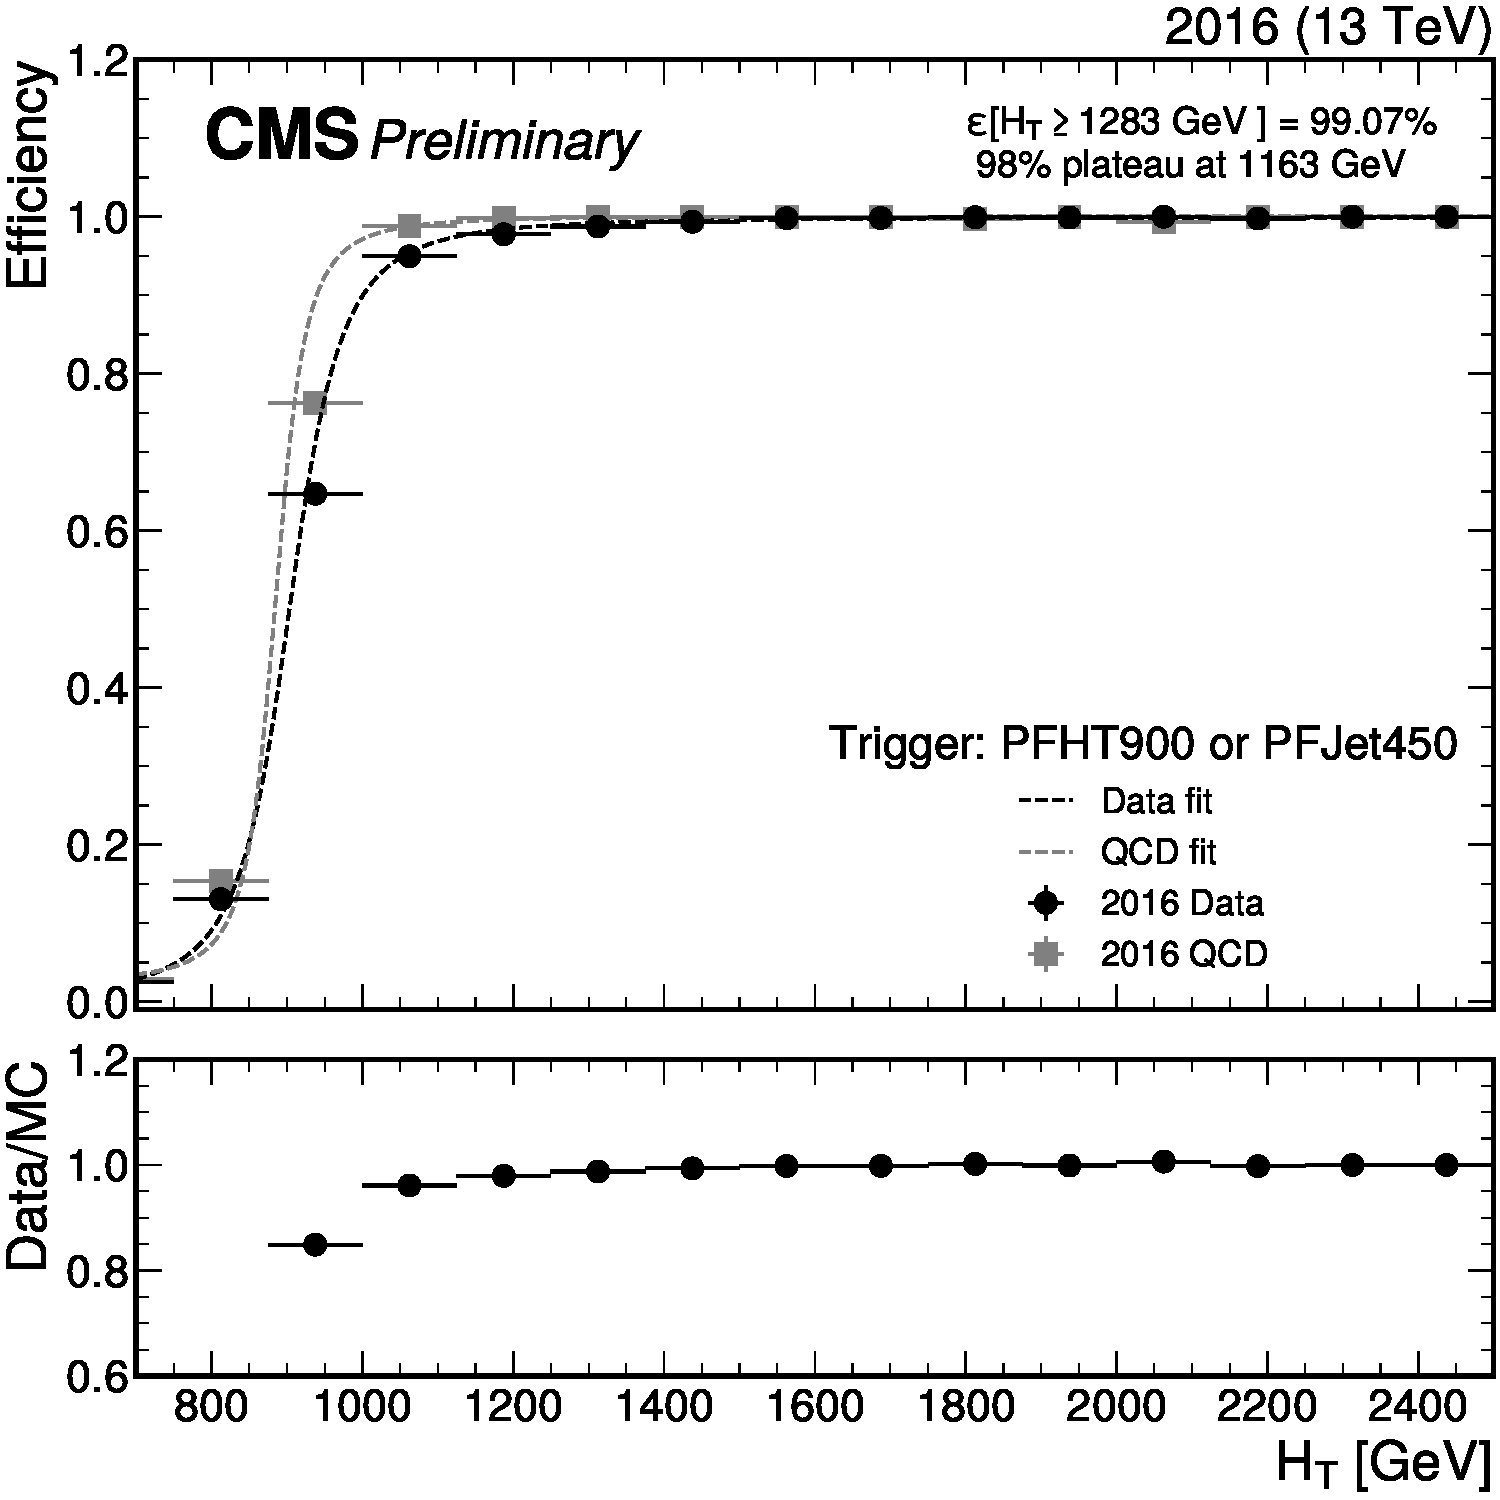
\includegraphics[width=\linewidth]{Images/pdfs/16_efficiency_withratio_and_fits.pdf}
		\caption{Run2 2016}
		\label{fig:HT_eff_16}
	\end{subfigure}
	%
	\begin{subfigure}{.45\textwidth}
		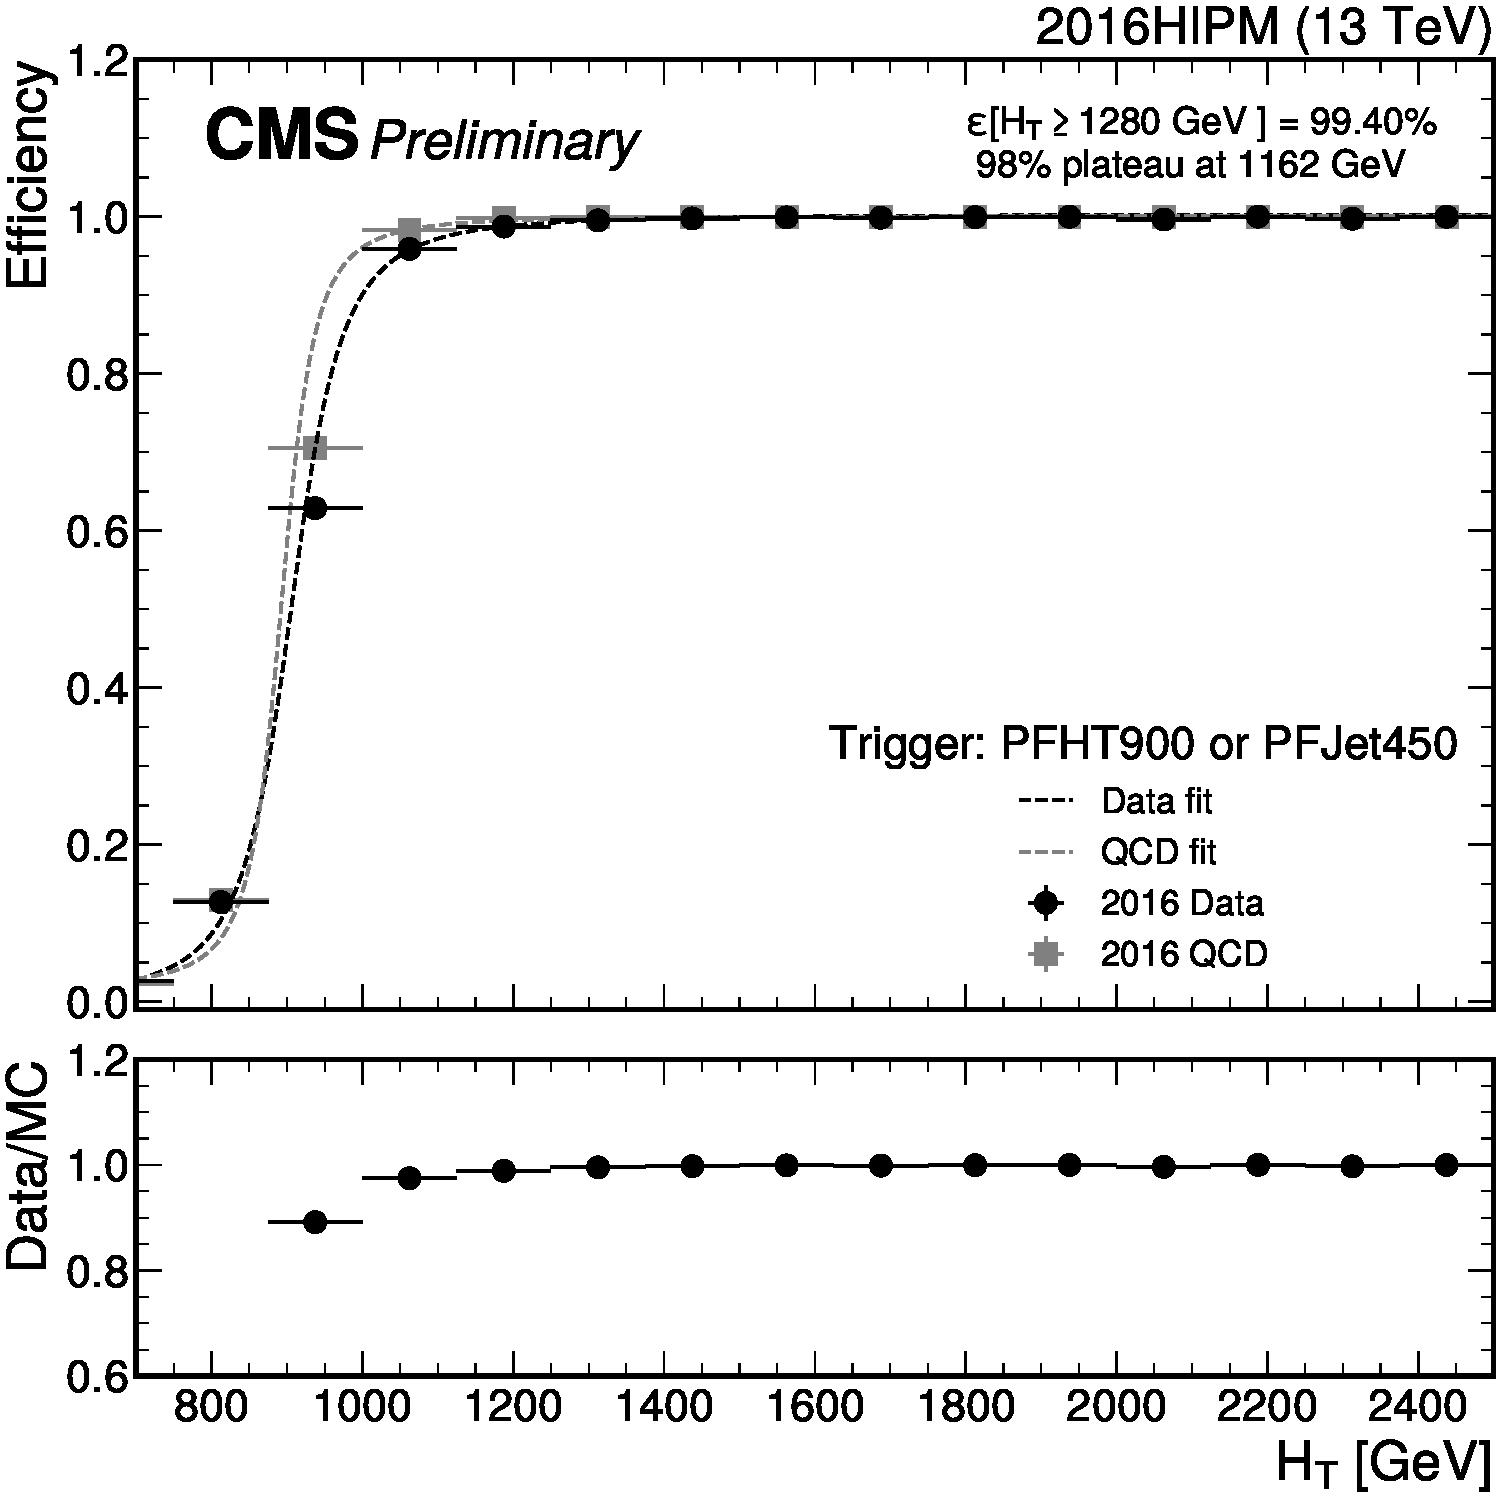
\includegraphics[width=\linewidth]{Images/pdfs/16-APV-HIPM_efficiency_withratio_and_fits.pdf}
		\caption{Run2 2016 HIPM}
		\label{fig:HT_eff_16_HIPM}
	\end{subfigure}

	\begin{subfigure}{.45\textwidth}
		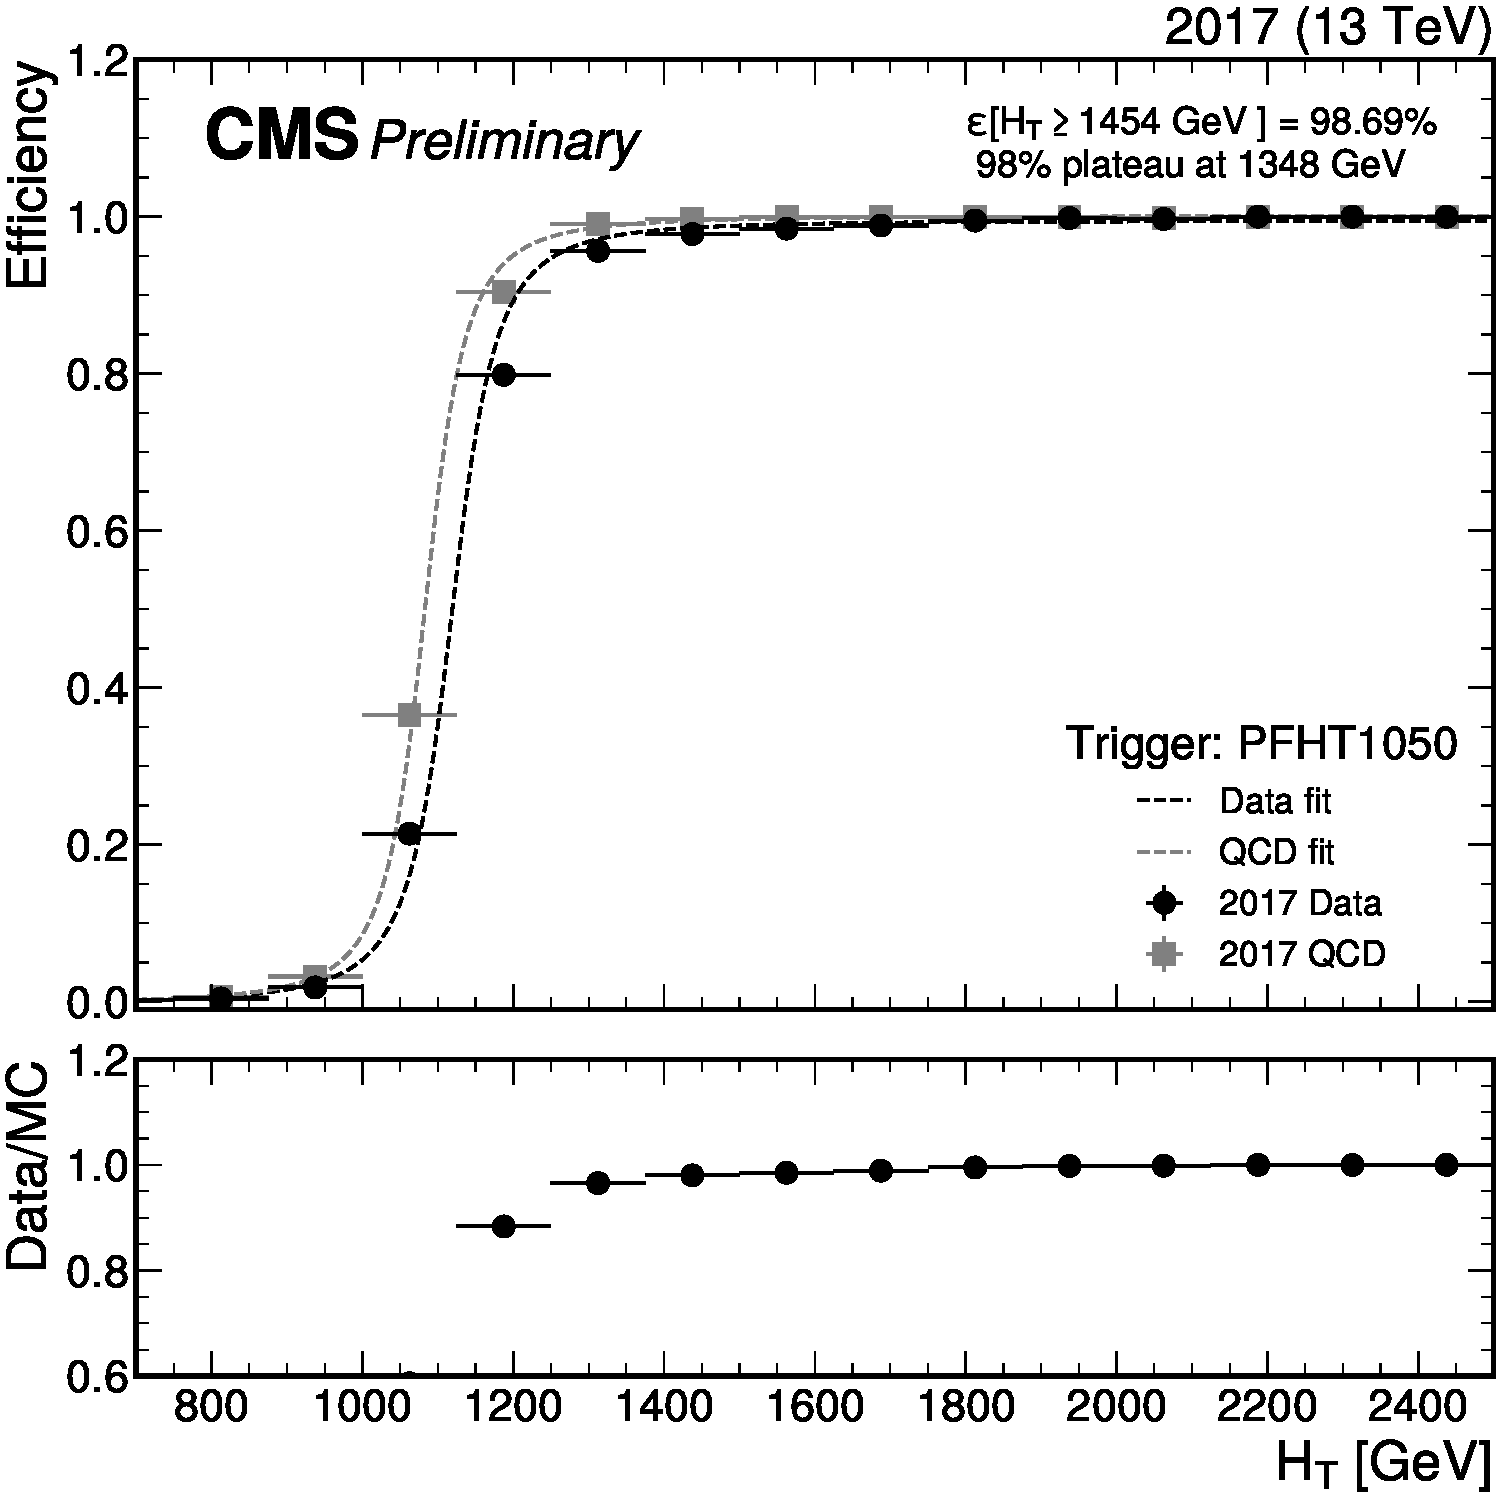
\includegraphics[width=\linewidth]{Images/pdfs/17_efficiency_withratio_and_fits.pdf}
		\caption{Run2 2017}
		\label{fig:HT_eff_17}
	\end{subfigure}
	%
	\begin{subfigure}{.45\textwidth}
		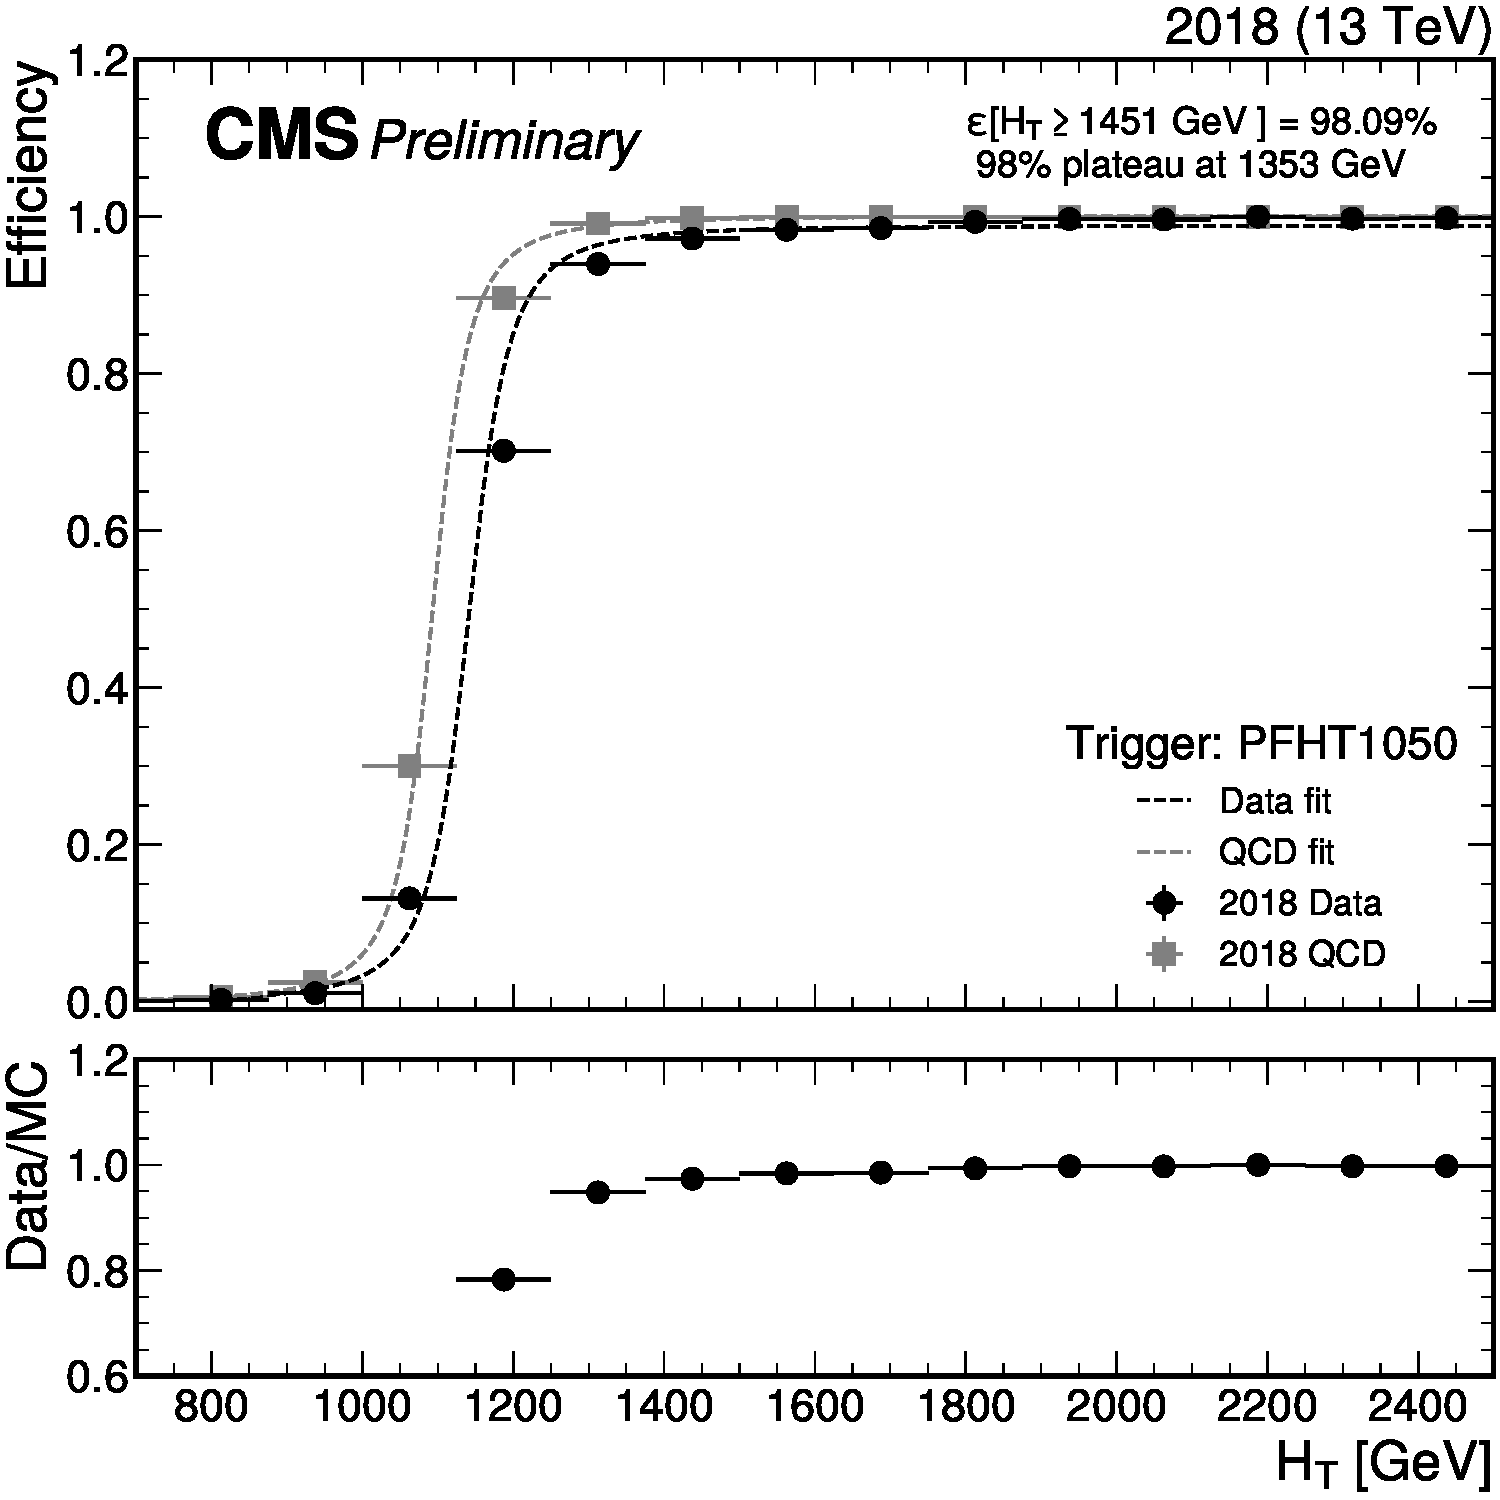
\includegraphics[width=\linewidth]{Images/pdfs/18_efficiency_withratio_and_fits.pdf}
		\caption{Run2 2018}
		\label{fig:HT_eff_18}
	\end{subfigure}
	\caption[Comparison of trigger efficiencies for \HT trigger]{Comparison of efficiency for \HT trigger as a function of event \HT measured relative to \texttt{HLT\_Mu50\_v*} in data (black) and QCD MC (gray) and fit to the algebraic function \textit{f} (line).}
	\label{fig:HT_efficiencies}
\end{figure}

The scale factor values used for signal MC can be found in \cref{tab:2016_triggerSF,tab:2016HIPM_triggerSF,tab:2017_triggerSF,tab:2018_triggerSF}. The uncertainties in the table are just the statistical uncertainties of data and MC selection efficiency propagated appropriately.


\begin{table}
	\centering
	\caption{Scale factors (SF) and statistical uncertainties of the \HT trigger for 2016.}
	\label{tab:2016_triggerSF}
	\begin{tabular}{cccc}
		\hline
		\HT bin[GeV]    & SF       & uncertainty (upper) & uncertainty (lower) \\
		\hline
		1200.0 - 1375.0 & 0.987578 & 0.001114            & 0.001227            \\
		1375.0 - 1500.0 & 0.993525 & 0.001043            & 0.001235            \\
		1500.0 - 1625.0 & 0.998121 & 0.000693            & 0.001015            \\
		1625.0 - 1750.0 & 0.998326 & 0.000801            & 0.001325            \\
		1750.0 - 1875.0 & 1.001928 & 0.000708            & 0.001671            \\
		1875.0 - 2000.0 & 0.998974 & 0.000848            & 0.002358            \\
		2000.0 - 2125.0 & 1.006414 & 0.000855            & 0.002898            \\
		2125.0 - 2250.0 & 0.997732 & 0.001876            & 0.005197            \\
		2250.0 - 2375.0 & 1.000000 & 0.000000            & 0.006580            \\
		2375.0 - 2500.0 & 1.000000 & 0.000000            & 0.009449            \\
		\hline
	\end{tabular}
\end{table}

\begin{table}
	\centering
	\caption{Scale factors (SF) and statistical uncertainties of the \HT trigger for 2016HIPM.}
	\label{tab:2016HIPM_triggerSF}
	\begin{tabular}{cccc}
		\hline
		\HT bin[GeV]    & SF       & uncertainty (upper) & uncertainty (lower) \\
		\hline
		1200.0 - 1375.0 & 0.995561 & 0.000618            & 0.000723            \\
		1375.0 - 1500.0 & 0.997767 & 0.000536            & 0.000697            \\
		1500.0 - 1625.0 & 0.999147 & 0.000408            & 0.000682            \\
		1625.0 - 1750.0 & 0.998692 & 0.000626            & 0.001037            \\
		1750.0 - 1875.0 & 0.999505 & 0.000410            & 0.001143            \\
		1875.0 - 2000.0 & 1.000000 & 0.000000            & 0.001484            \\
		2000.0 - 2125.0 & 0.996381 & 0.001969            & 0.003510            \\
		2125.0 - 2250.0 & 1.000000 & 0.000000            & 0.003497            \\
		2250.0 - 2375.0 & 0.997389 & 0.002160            & 0.005981            \\
		2375.0 - 2500.0 & 1.000000 & 0.000000            & 0.006582            \\
		\hline
	\end{tabular}
\end{table}

\begin{table}
	\centering
	\caption{Scale factors and statistical uncertainties of the \HT trigger for 2017.}
	\label{tab:2017_triggerSF}
	\begin{tabular}{cccc}
		\hline
		\HT bin[GeV]    & SF       & uncertainty (upper) & uncertainty (lower) \\
		\hline
		1200.0 - 1375.0 & 0.965681 & 0.001357            & 0.001412            \\
		1375.0 - 1500.0 & 0.980217 & 0.001125            & 0.001199            \\
		1500.0 - 1625.0 & 0.985178 & 0.001111            & 0.001201            \\
		1625.0 - 1750.0 & 0.989094 & 0.001191            & 0.001328            \\
		1750.0 - 1875.0 & 0.995385 & 0.000992            & 0.001215            \\
		1875.0 - 2000.0 & 0.998218 & 0.000735            & 0.001111            \\
		2000.0 - 2125.0 & 0.998595 & 0.001134            & 0.001635            \\
		2125.0 - 2250.0 & 1.000000 & 0.000000            & 0.001187            \\
		2250.0 - 2375.0 & 1.000000 & 0.000000            & 0.001821            \\
		2375.0 - 2500.0 & 1.000277 & 0.000166            & 0.002397            \\
		2500.0 - 2625.0 & 1.005464 & 0.001036            & 0.003895            \\
		\hline
	\end{tabular}
\end{table}

\begin{table}
	\centering
	\caption{Scale factors and statistical uncertainties of the \HT trigger for 2018.}
	\label{tab:2018_triggerSF}
	\begin{tabular}{cccc}
		\hline
		\HT bin[GeV]    & SF       & uncertainty (upper) & uncertainty (lower) \\
		\hline
		1200.0 - 1375.0 & 0.947967 & 0.001657            & 0.001723            \\
		1375.0 - 1500.0 & 0.973940 & 0.001332            & 0.001409            \\
		1500.0 - 1625.0 & 0.983915 & 0.001286            & 0.001392            \\
		1625.0 - 1750.0 & 0.985506 & 0.001518            & 0.001685            \\
		1750.0 - 1875.0 & 0.993555 & 0.001249            & 0.001515            \\
		1875.0 - 2000.0 & 0.997541 & 0.001054            & 0.001498            \\
		2000.0 - 2125.0 & 0.997264 & 0.001403            & 0.002103            \\
		2125.0 - 2250.0 & 1.000000 & 0.000000            & 0.001596            \\
		2250.0 - 2375.0 & 0.997558 & 0.001577            & 0.003217            \\
		2375.0 - 2500.0 & 0.998141 & 0.001538            & 0.004268            \\
		\hline
	\end{tabular}
\end{table}

For completeness we also checked the trigger efficiencies in a region of phase-space were we expect to be signal-free (i.e. SinglePhoton data stream). We see in a similar fashion the plots for these unprescaled triggers divided by year in \cref{fig:HT_eff_SinglePhoton_16,fig:HT_eff_SinglePhoton_16_HIPM,fig:HT_eff_SinglePhoton_17,fig:HT_eff_SinglePhoton_18}.
More detailed plots of the fit functions around the turn-on region can be found in \cref{fig:fits}
that show the $H_T$ trigger efficiencies in each fit.



\begin{figure}
	\centering
	\begin{subfigure}{.45\textwidth}
		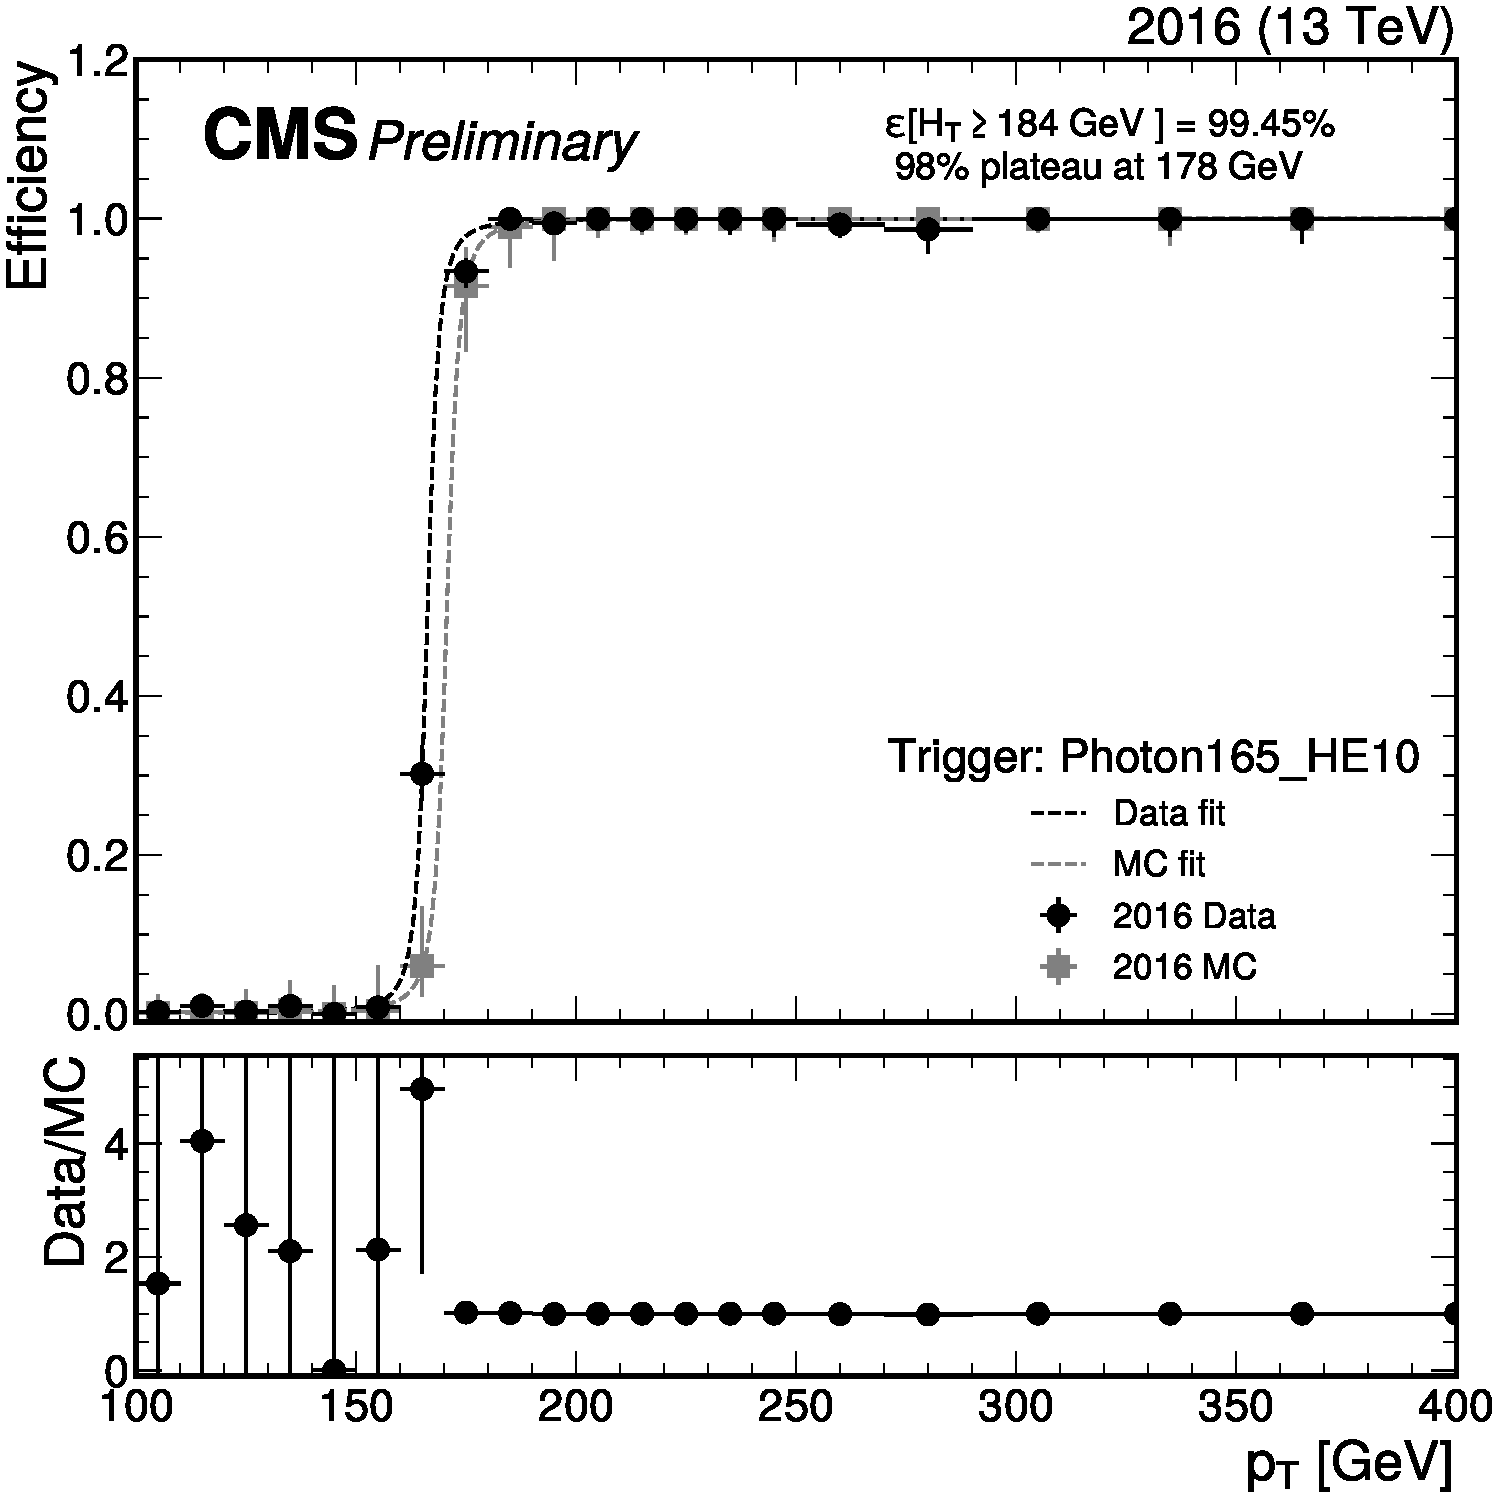
\includegraphics[width=\linewidth]{Images/pdfs/16_SinglePhoton_efficiency_withratio_and_fits.pdf}
		\caption{Run2 SinglePhoton 2016}
		\label{fig:HT_eff_SinglePhoton_16}
	\end{subfigure}
	%
	\begin{subfigure}{.45\textwidth}
		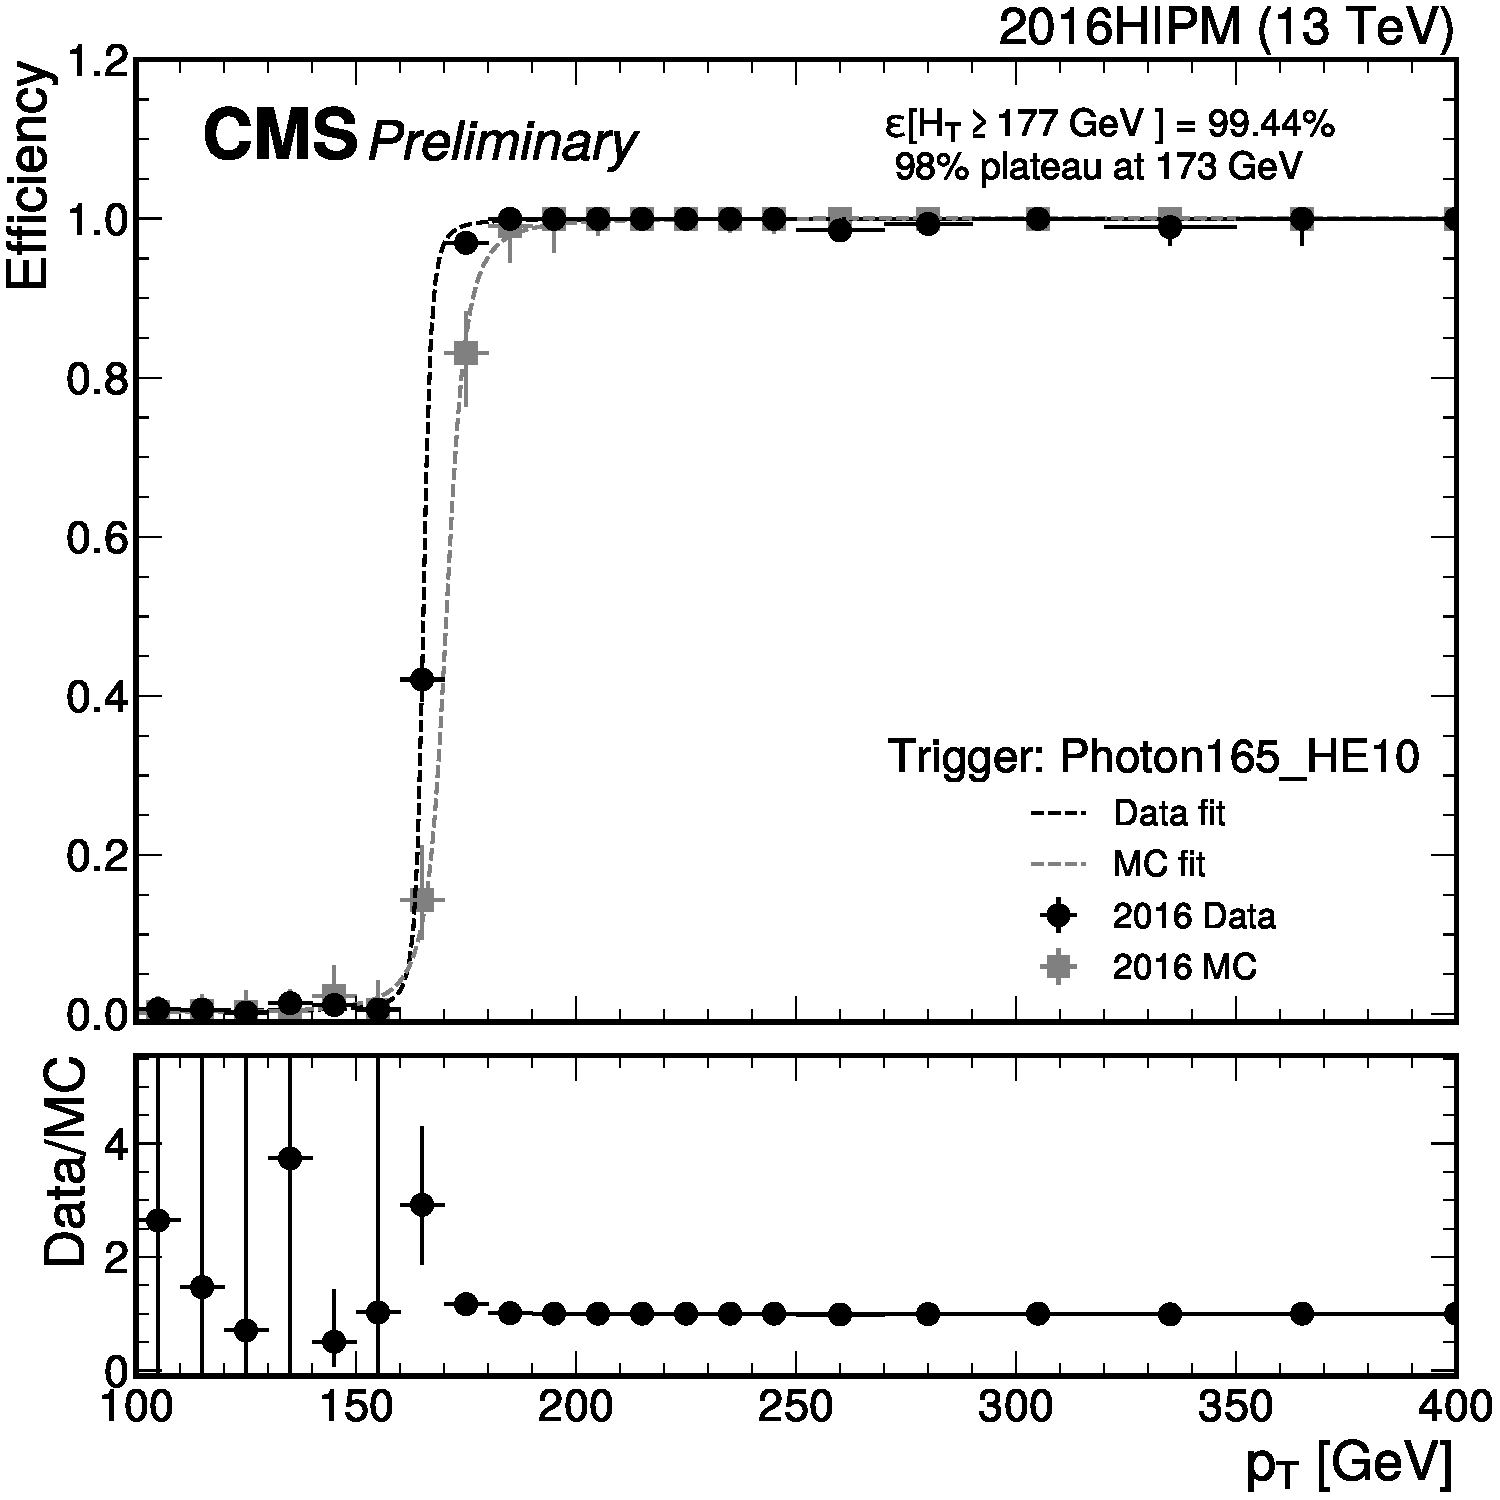
\includegraphics[width=\linewidth]{Images/pdfs/16-APV-HIPM_SinglePhoton_efficiency_withratio_and_fits.pdf}
		\caption{Run2 SinglePhoton 2016 HIPM}
		\label{fig:HT_eff_SinglePhoton_16_HIPM}
	\end{subfigure}

	\begin{subfigure}{.45\textwidth}
		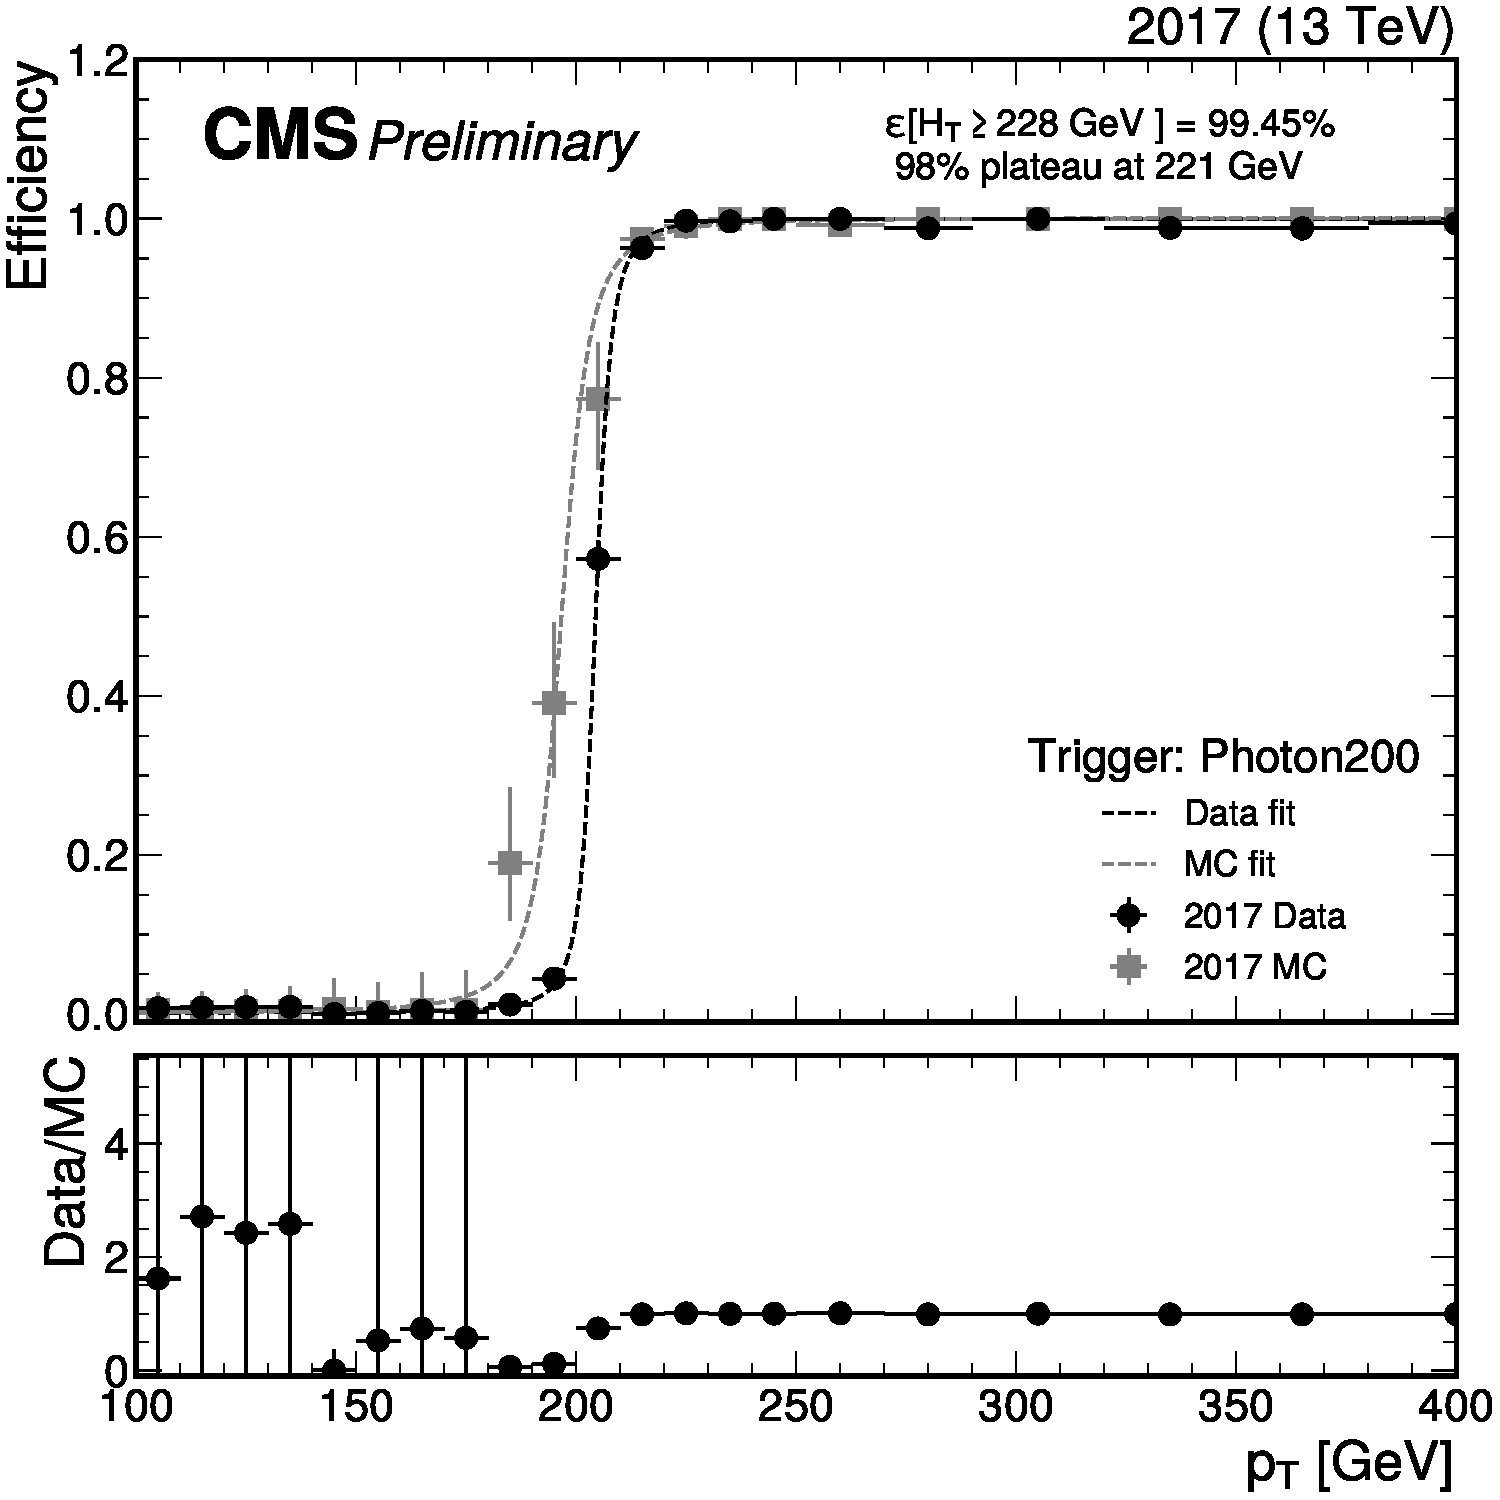
\includegraphics[width=\linewidth]{Images/pdfs/17_SinglePhoton_efficiency_withratio_and_fits.pdf}
		\caption{Run2 SinglePhoton 2017}
		\label{fig:HT_eff_SinglePhoton_17}
	\end{subfigure}
	%
	\begin{subfigure}{.45\textwidth}
		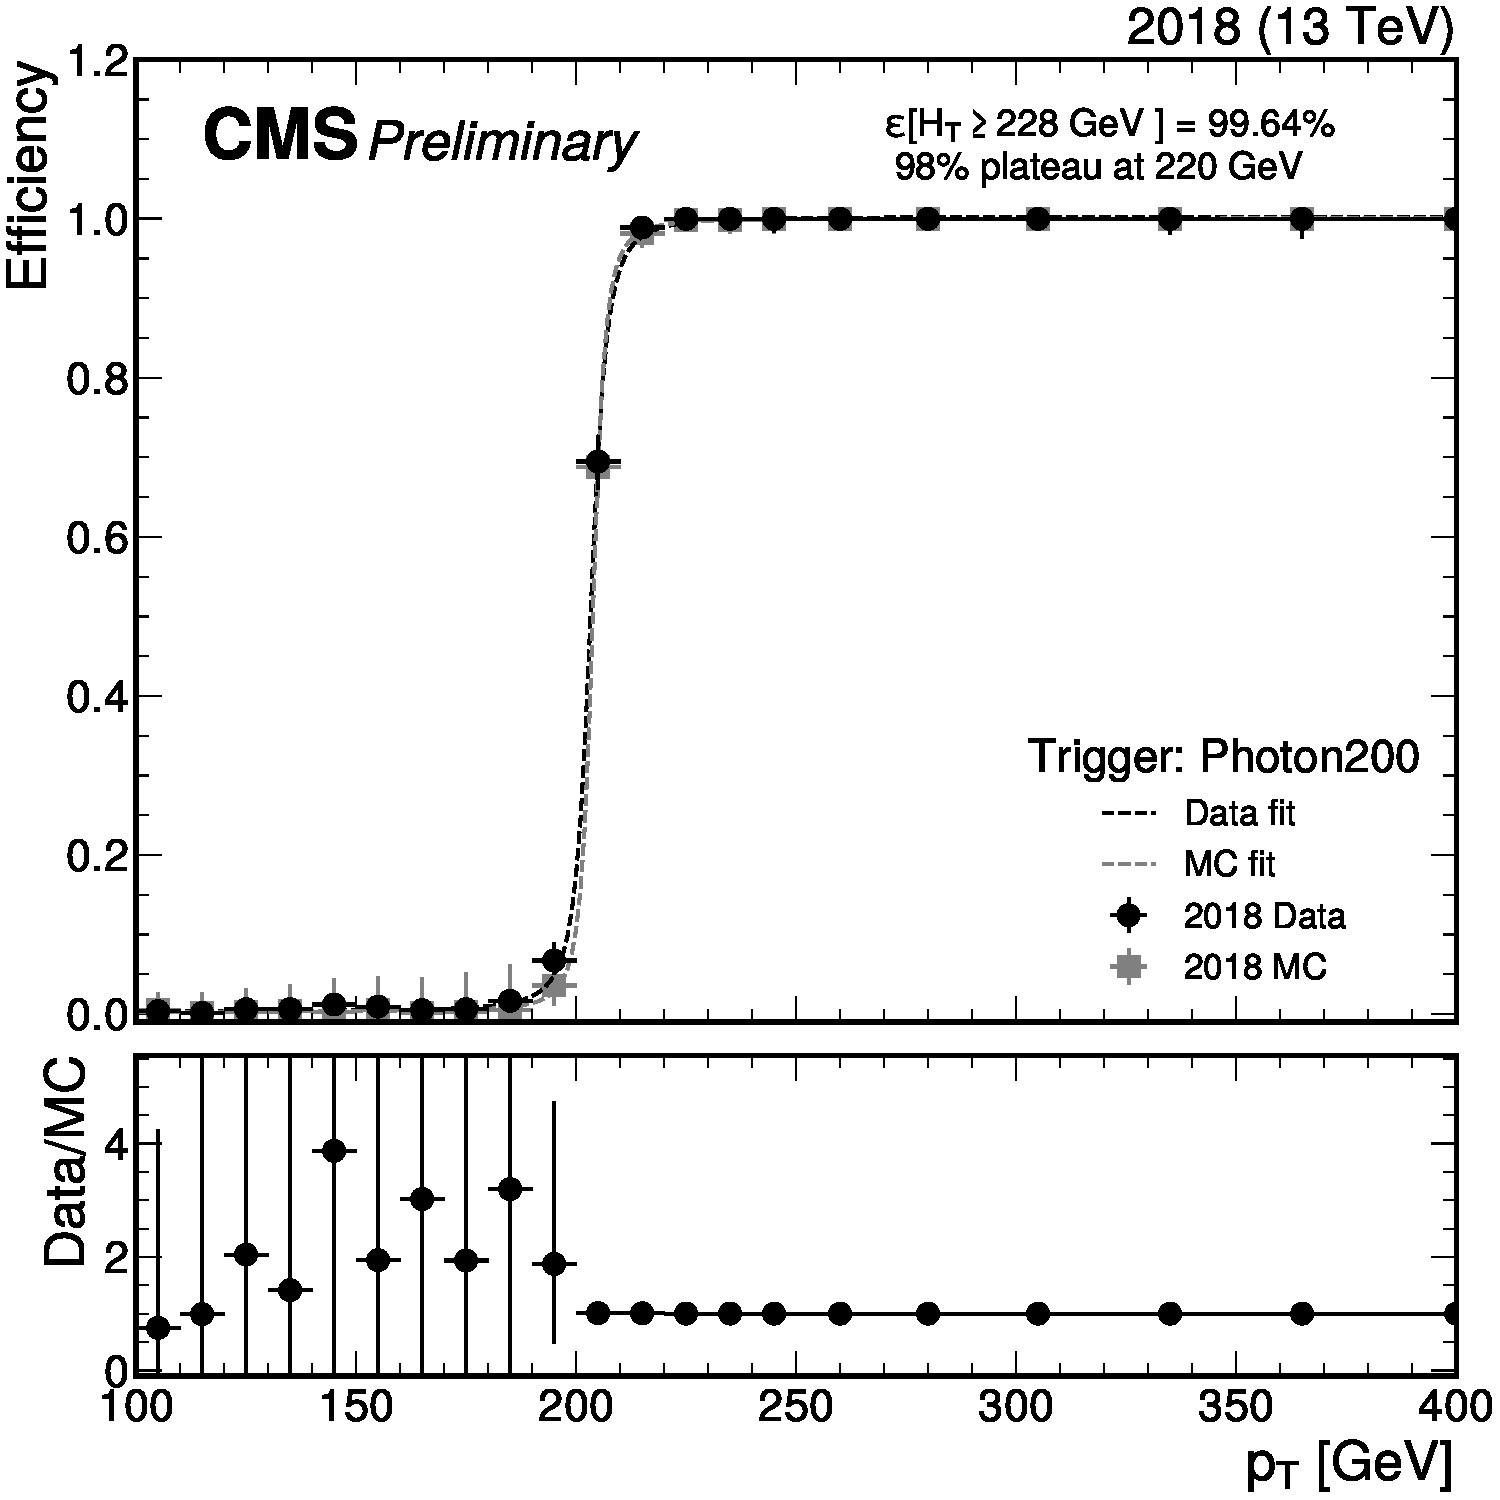
\includegraphics[width=\linewidth]{Images/pdfs/18_SinglePhoton_efficiency_withratio_and_fits.pdf}
		\caption{Run2 SinglePhoton 2018}
		\label{fig:HT_eff_SinglePhoton_18}
	\end{subfigure}
	\caption[Comparison of trigger efficiencies for \HT trigger for the signal free region.]{Comparison of efficiency for $p_T$ trigger as a function of  jet $p_T$ for the SinglePhoton data stream. Measured relative to \texttt{HLT\_Mu50\_v*} in data (black) and QCD MC (gray) and fit to the algebraic function \textit{f} (line).}
\end{figure}


\begin{figure}
	\centering
	\begin{subfigure}{.36\linewidth}
		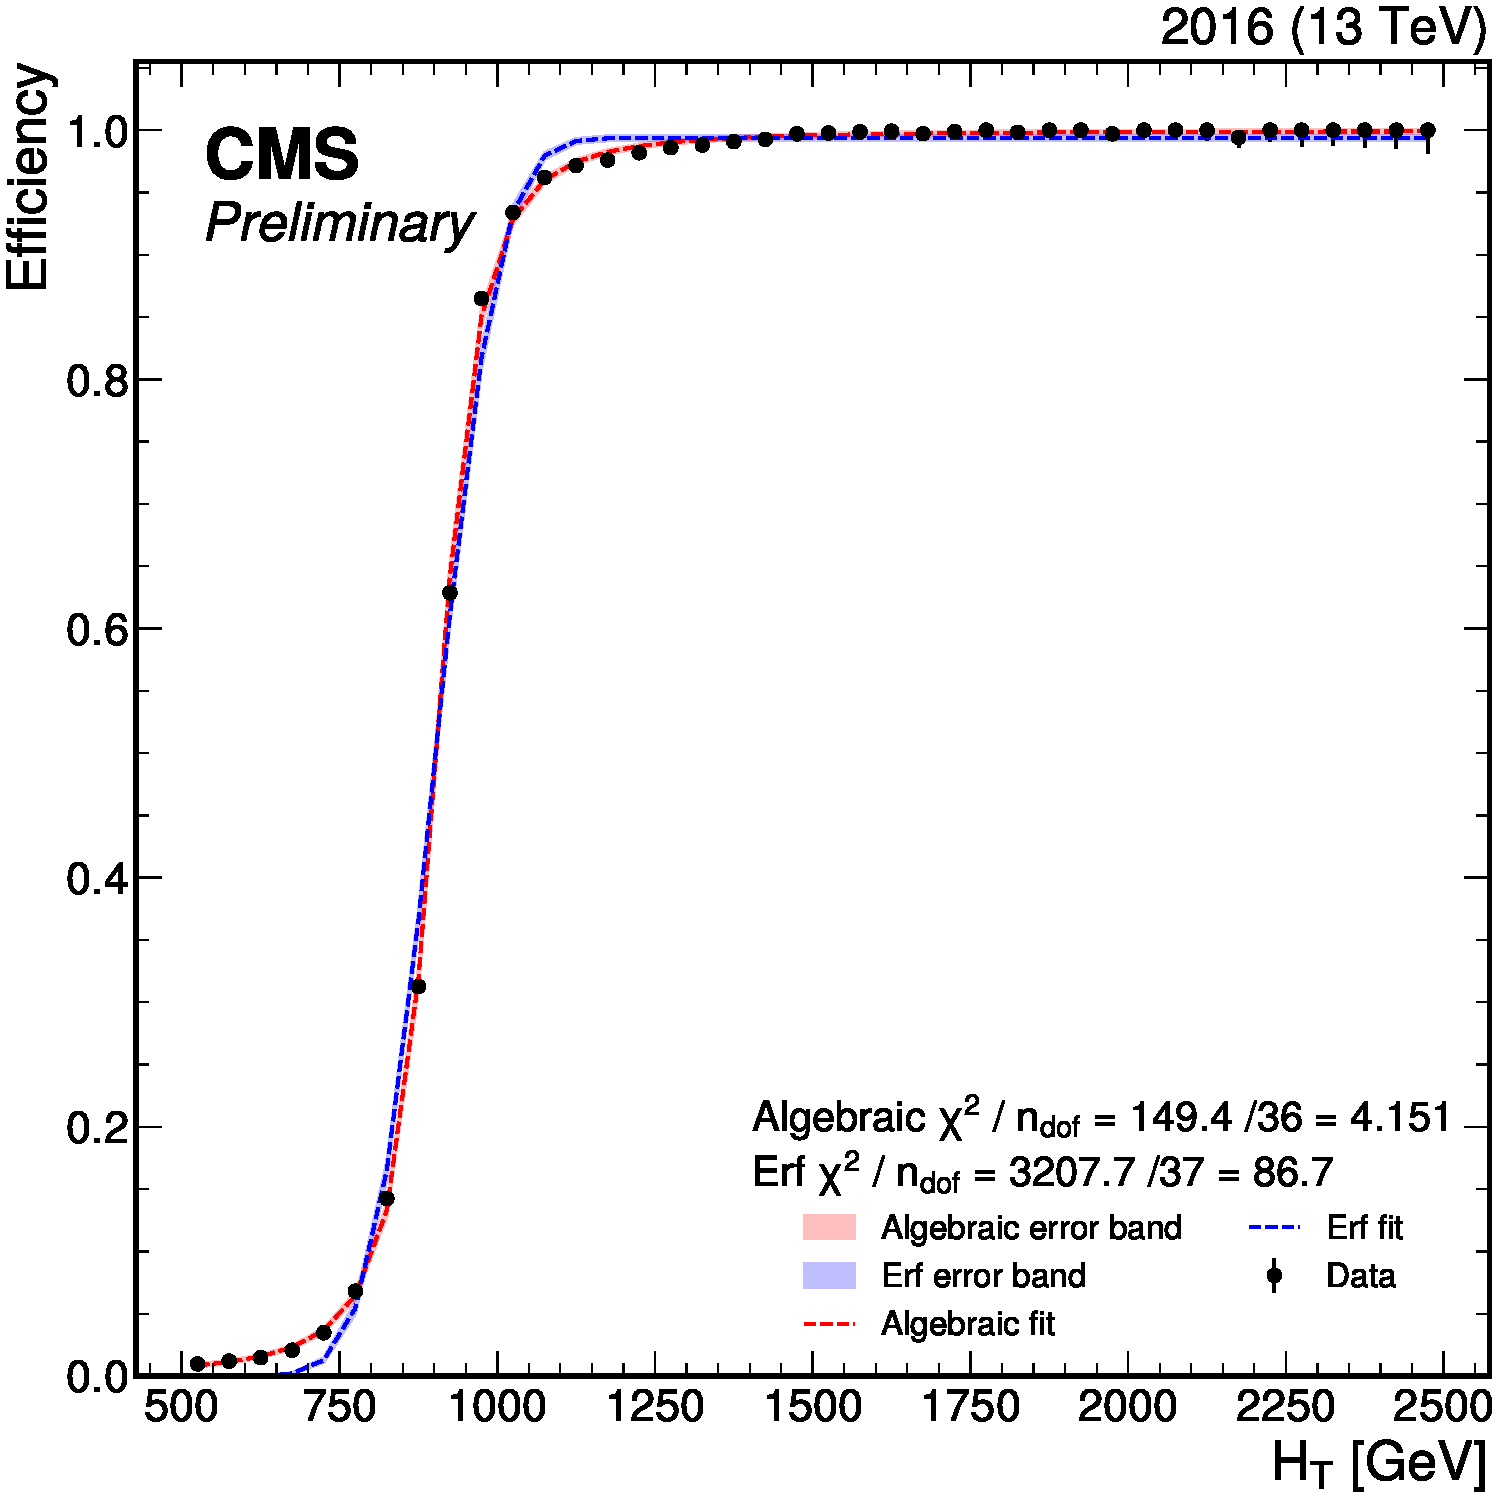
\includegraphics[width=\linewidth]{Images/pdfs/fits_16.pdf}
		% \caption{Caption}
		% \label{fig:enter-label}
	\end{subfigure}%
	\begin{subfigure}{.36\linewidth}
		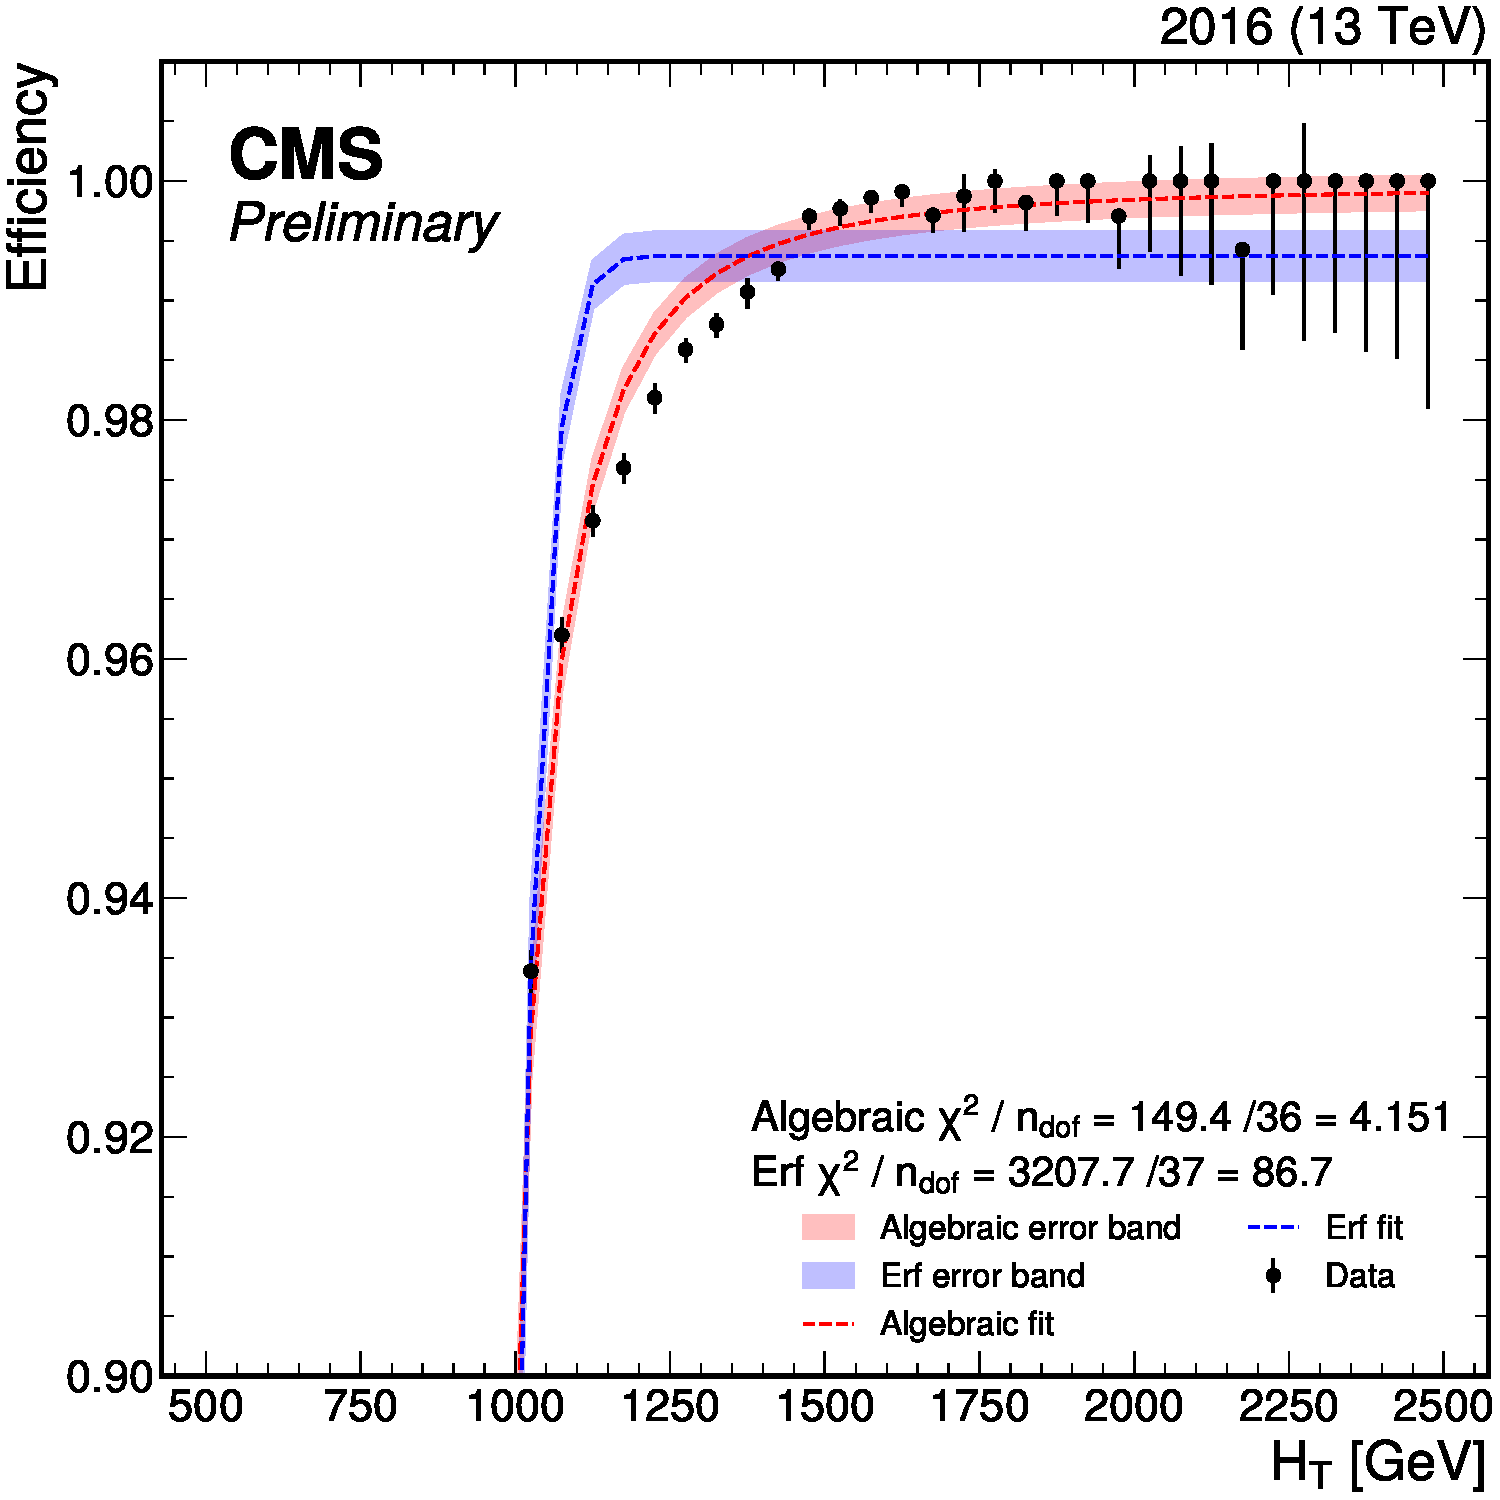
\includegraphics[width=\linewidth]{Images/pdfs/fits_closeup_16.pdf}
		% \caption{Caption}
		% \label{fig:enter-label}
	\end{subfigure}
	\begin{subfigure}{.36\linewidth}
		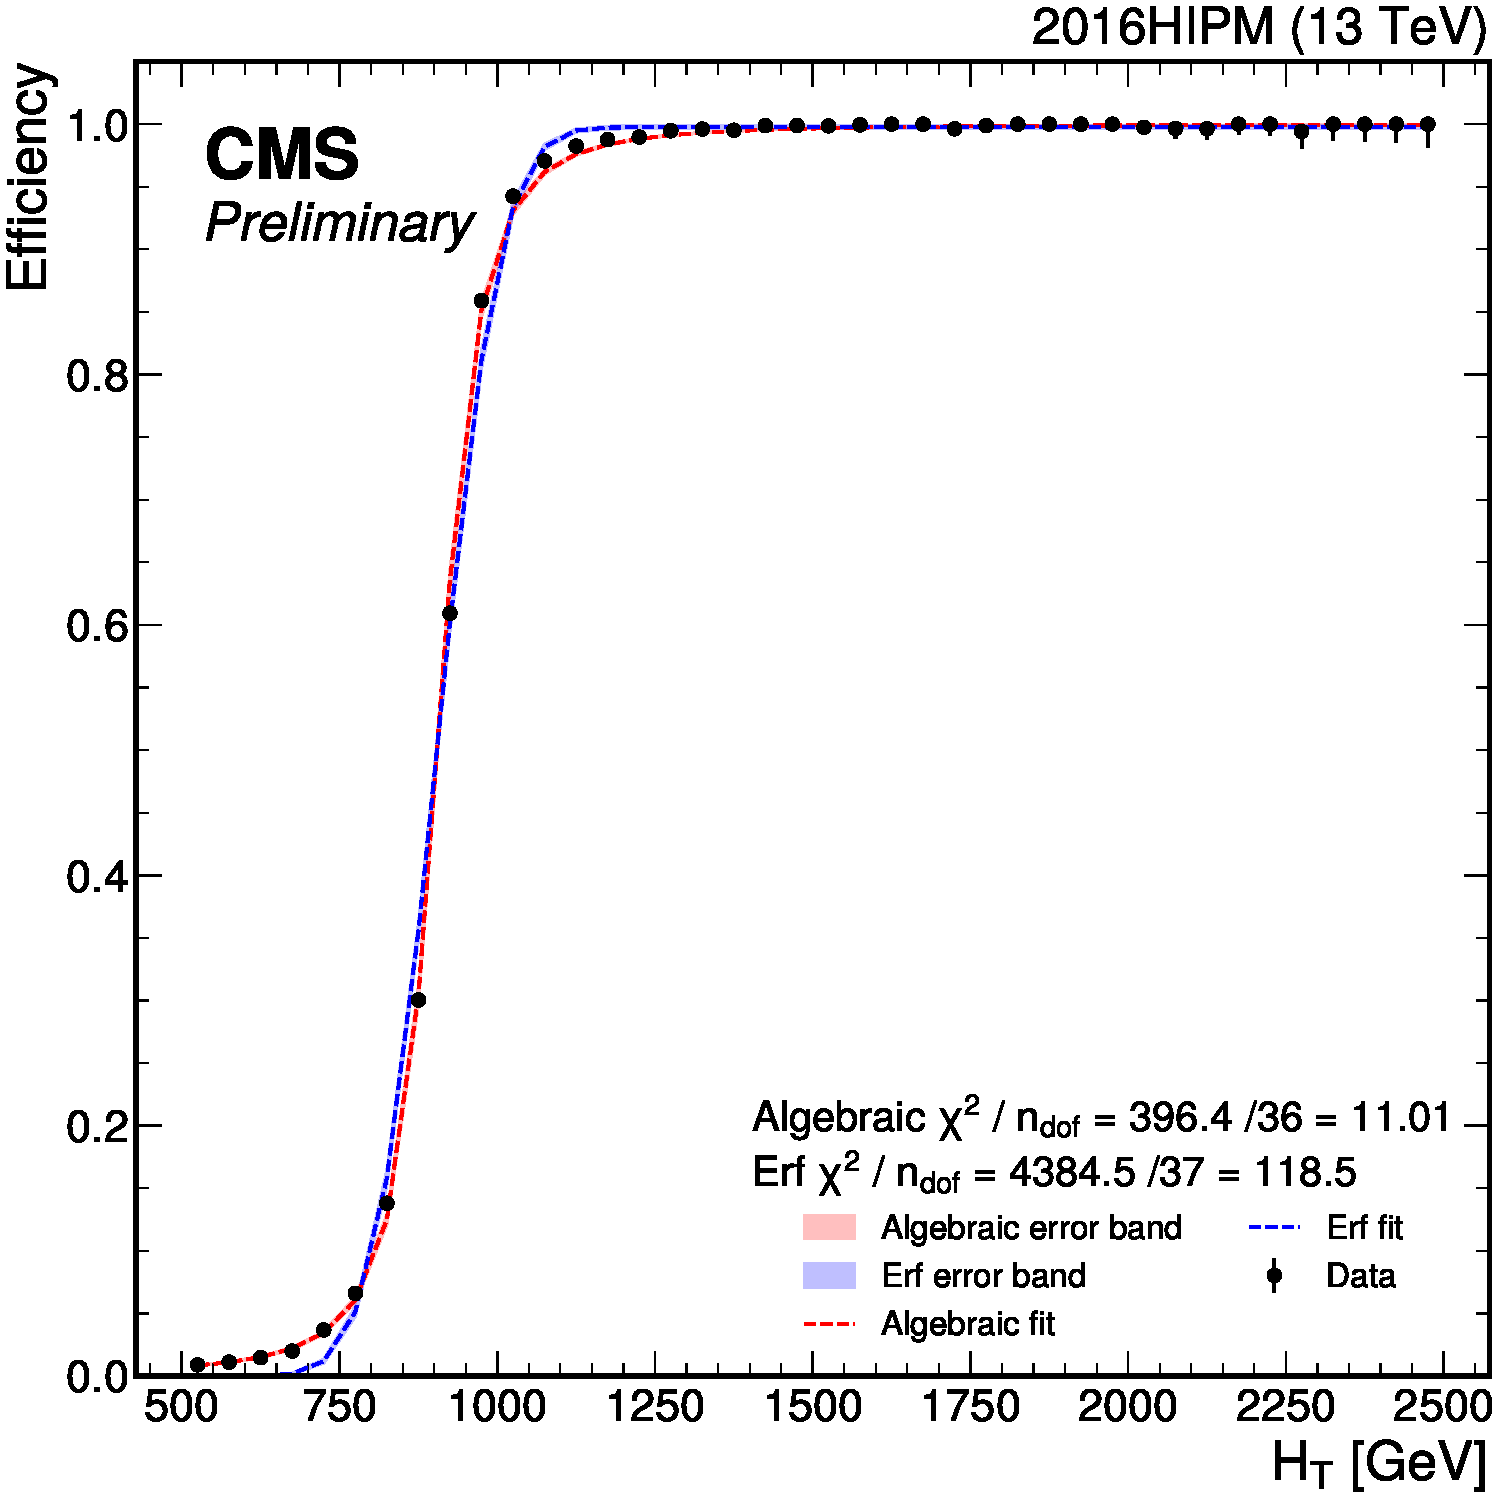
\includegraphics[width=\linewidth]{Images/pdfs/fits_16-APV-HIPM.pdf}
		% \caption{Caption}
		% \label{fig:enter-label}
	\end{subfigure}%
	\begin{subfigure}{.36\linewidth}
		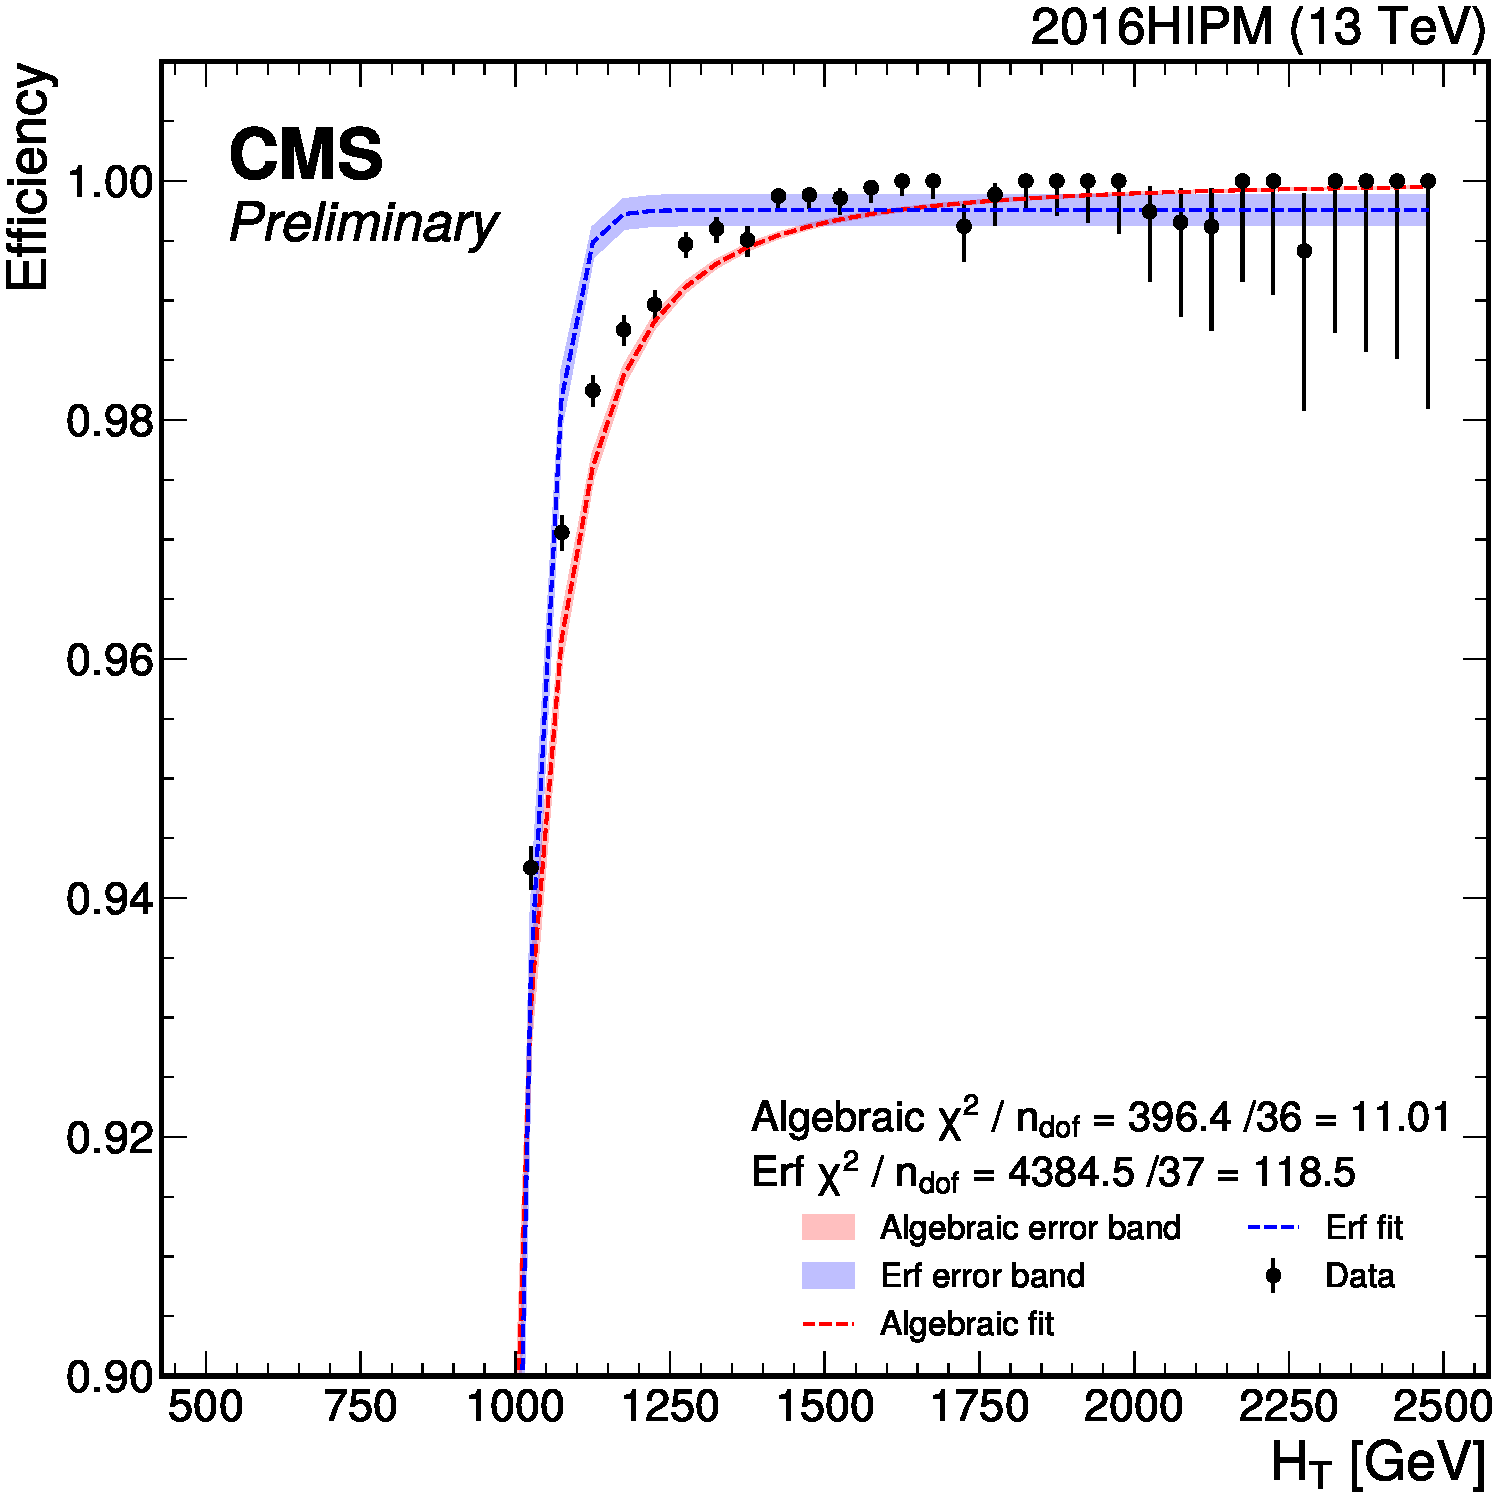
\includegraphics[width=\linewidth]{Images/pdfs/fits_closeup_16-APV-HIPM.pdf}
		% \caption{Caption}
		% \label{fig:enter-label}
	\end{subfigure}
	\begin{subfigure}{.36\linewidth}
		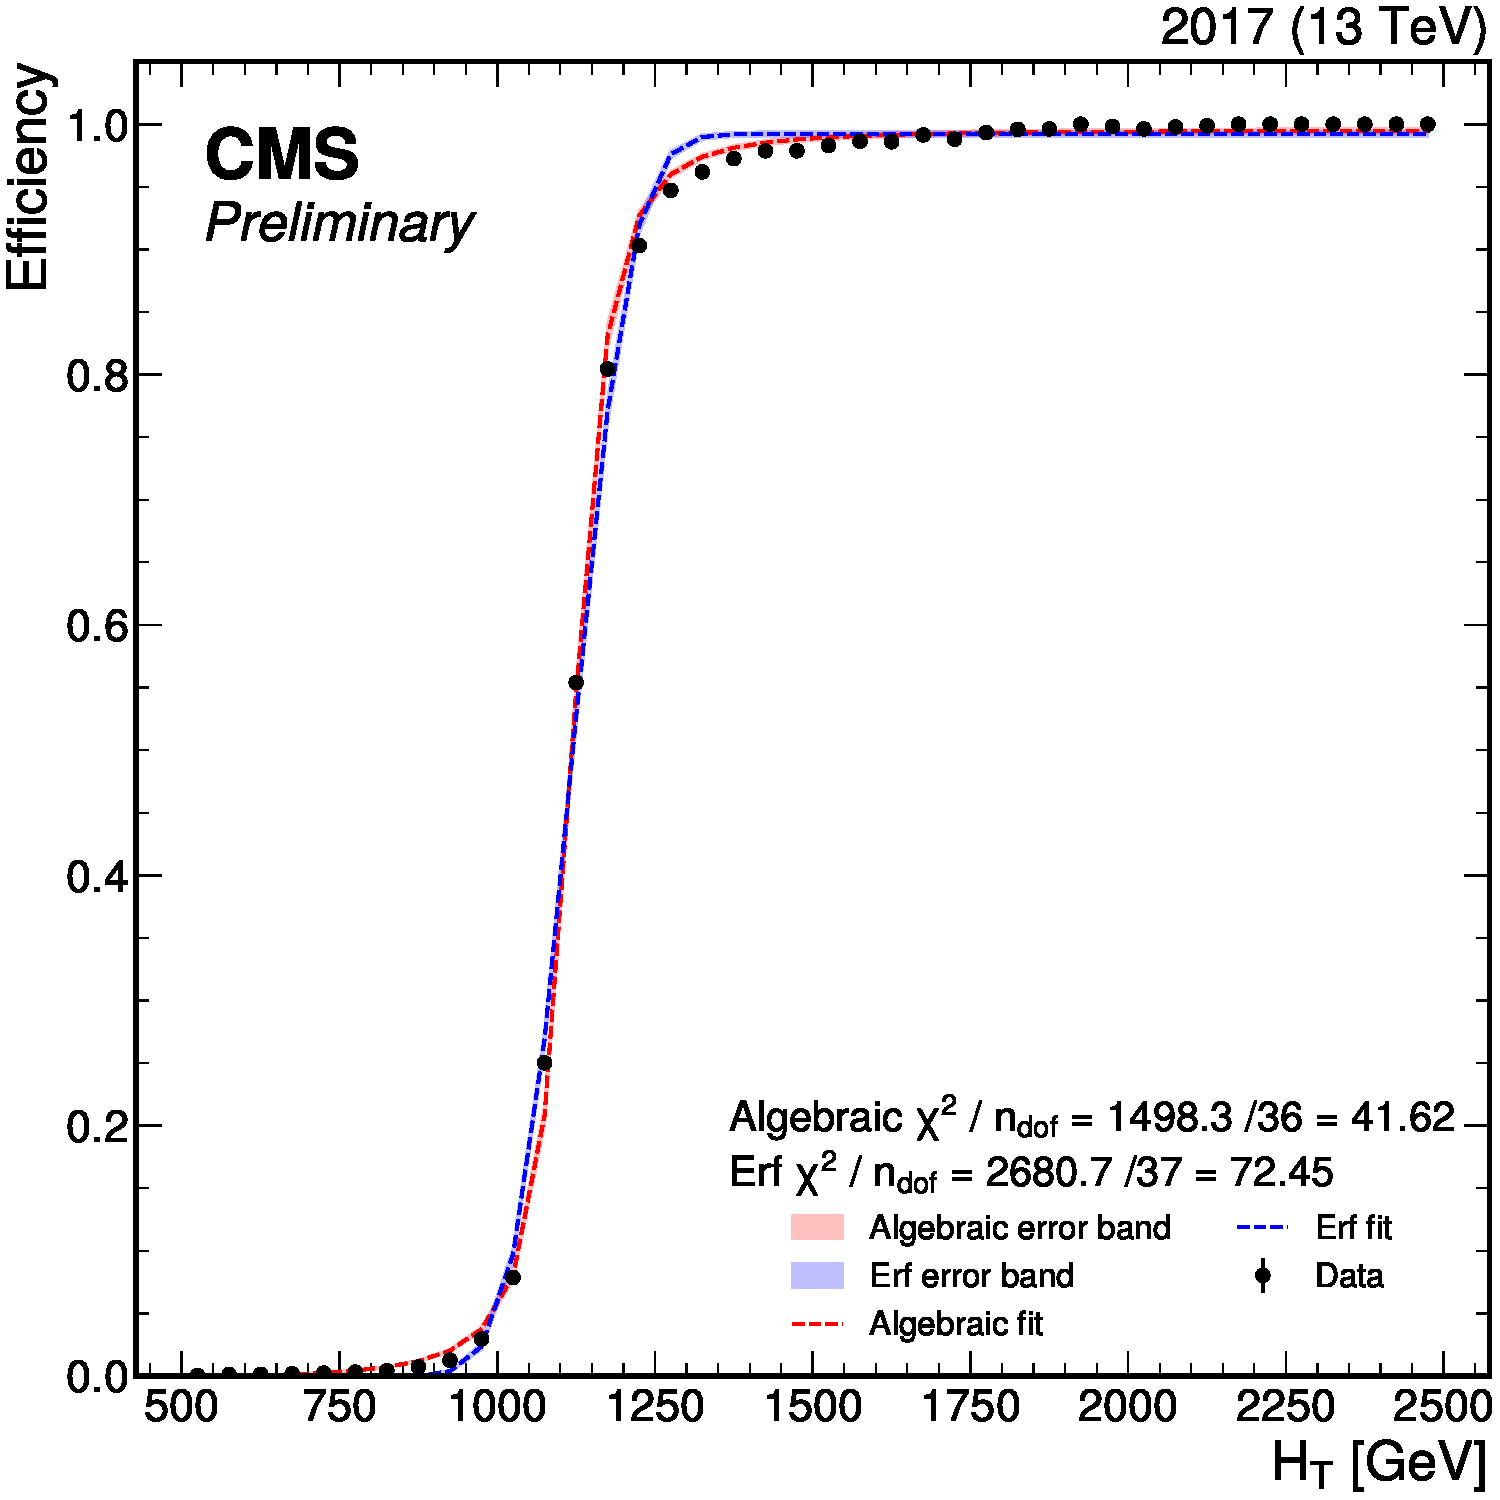
\includegraphics[width=\linewidth]{Images/pdfs/fits_17.pdf}
		% \caption{Caption}
		% \label{fig:enter-label}
	\end{subfigure}%
	\begin{subfigure}{.36\linewidth}
		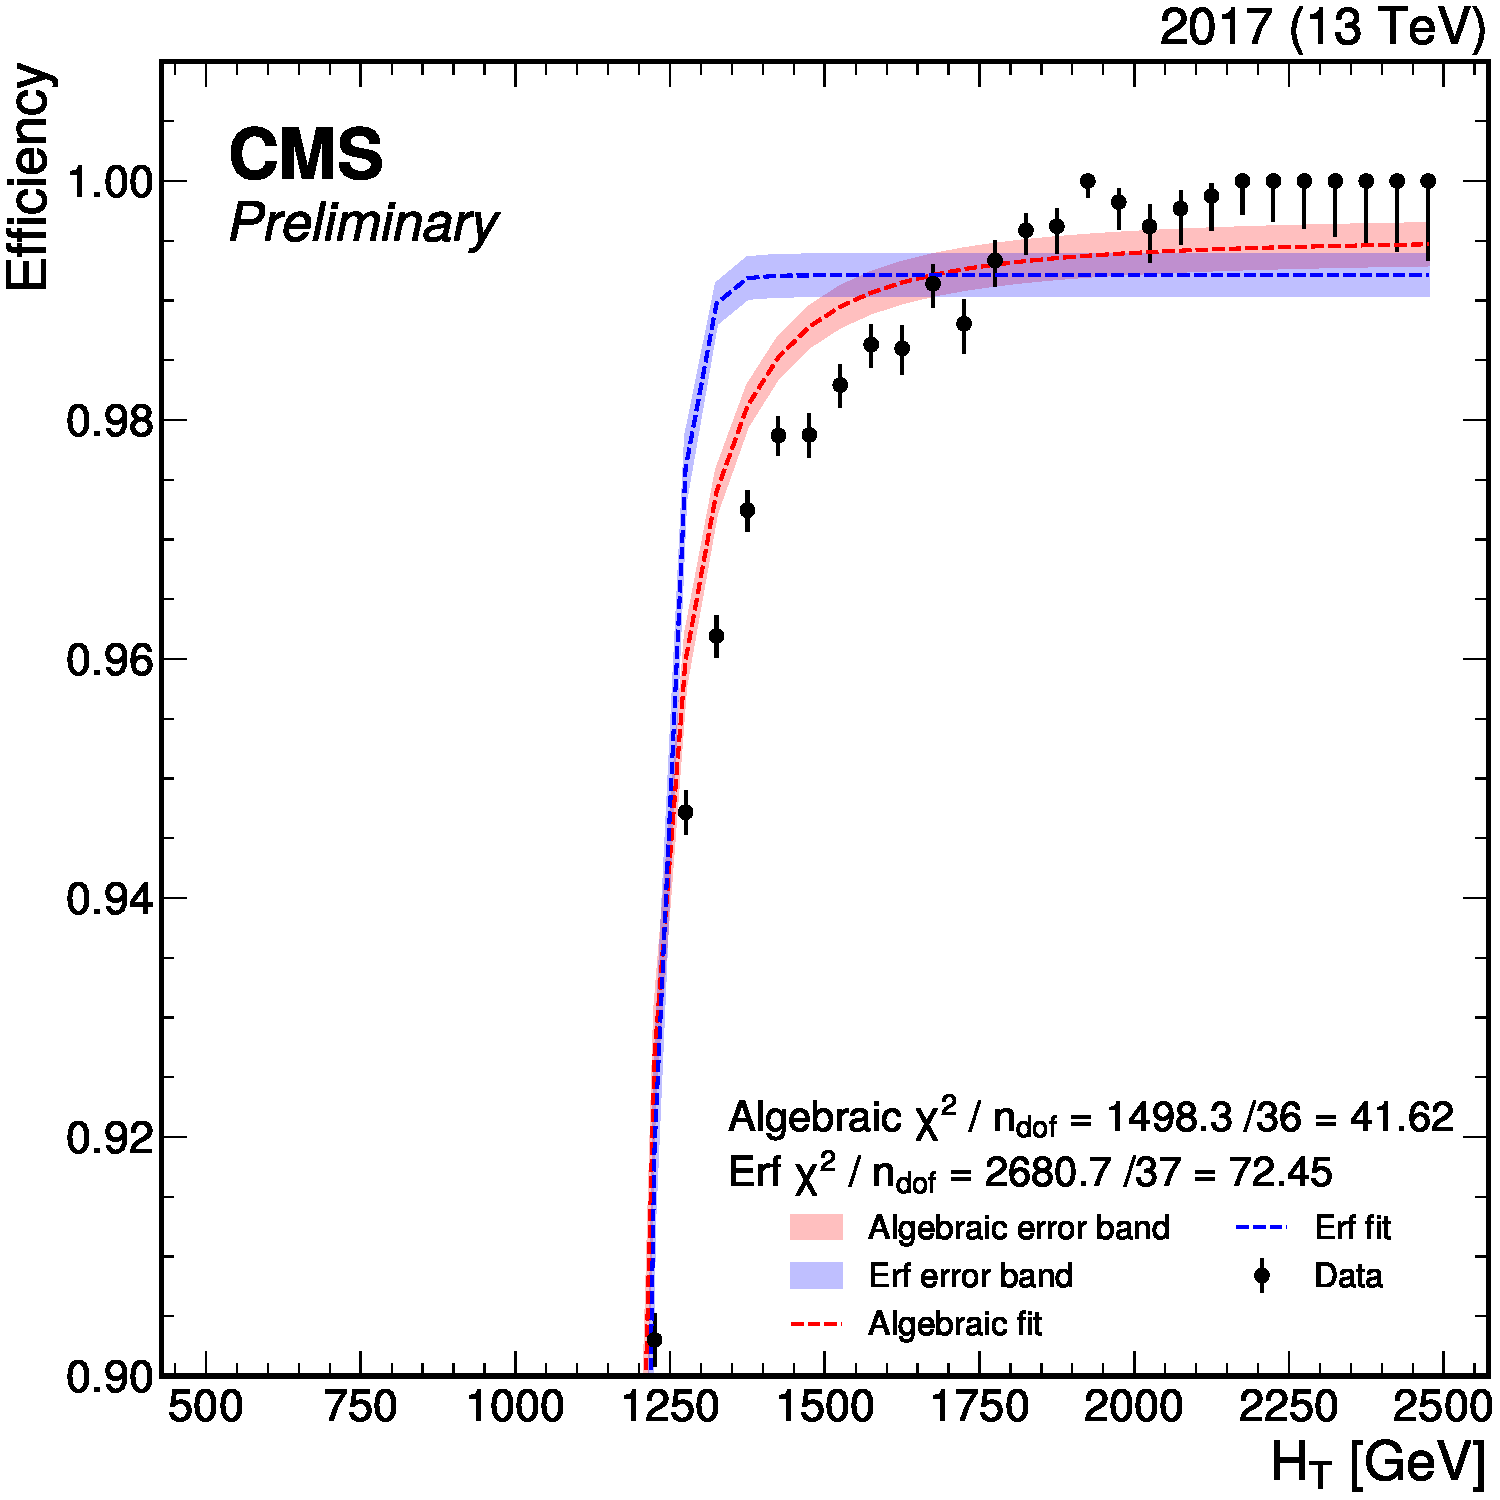
\includegraphics[width=\linewidth]{Images/pdfs/fits_closeup_17.pdf}
		% \caption{Caption}
		% \label{fig:enter-label}
	\end{subfigure}
	\begin{subfigure}{.36\linewidth}
		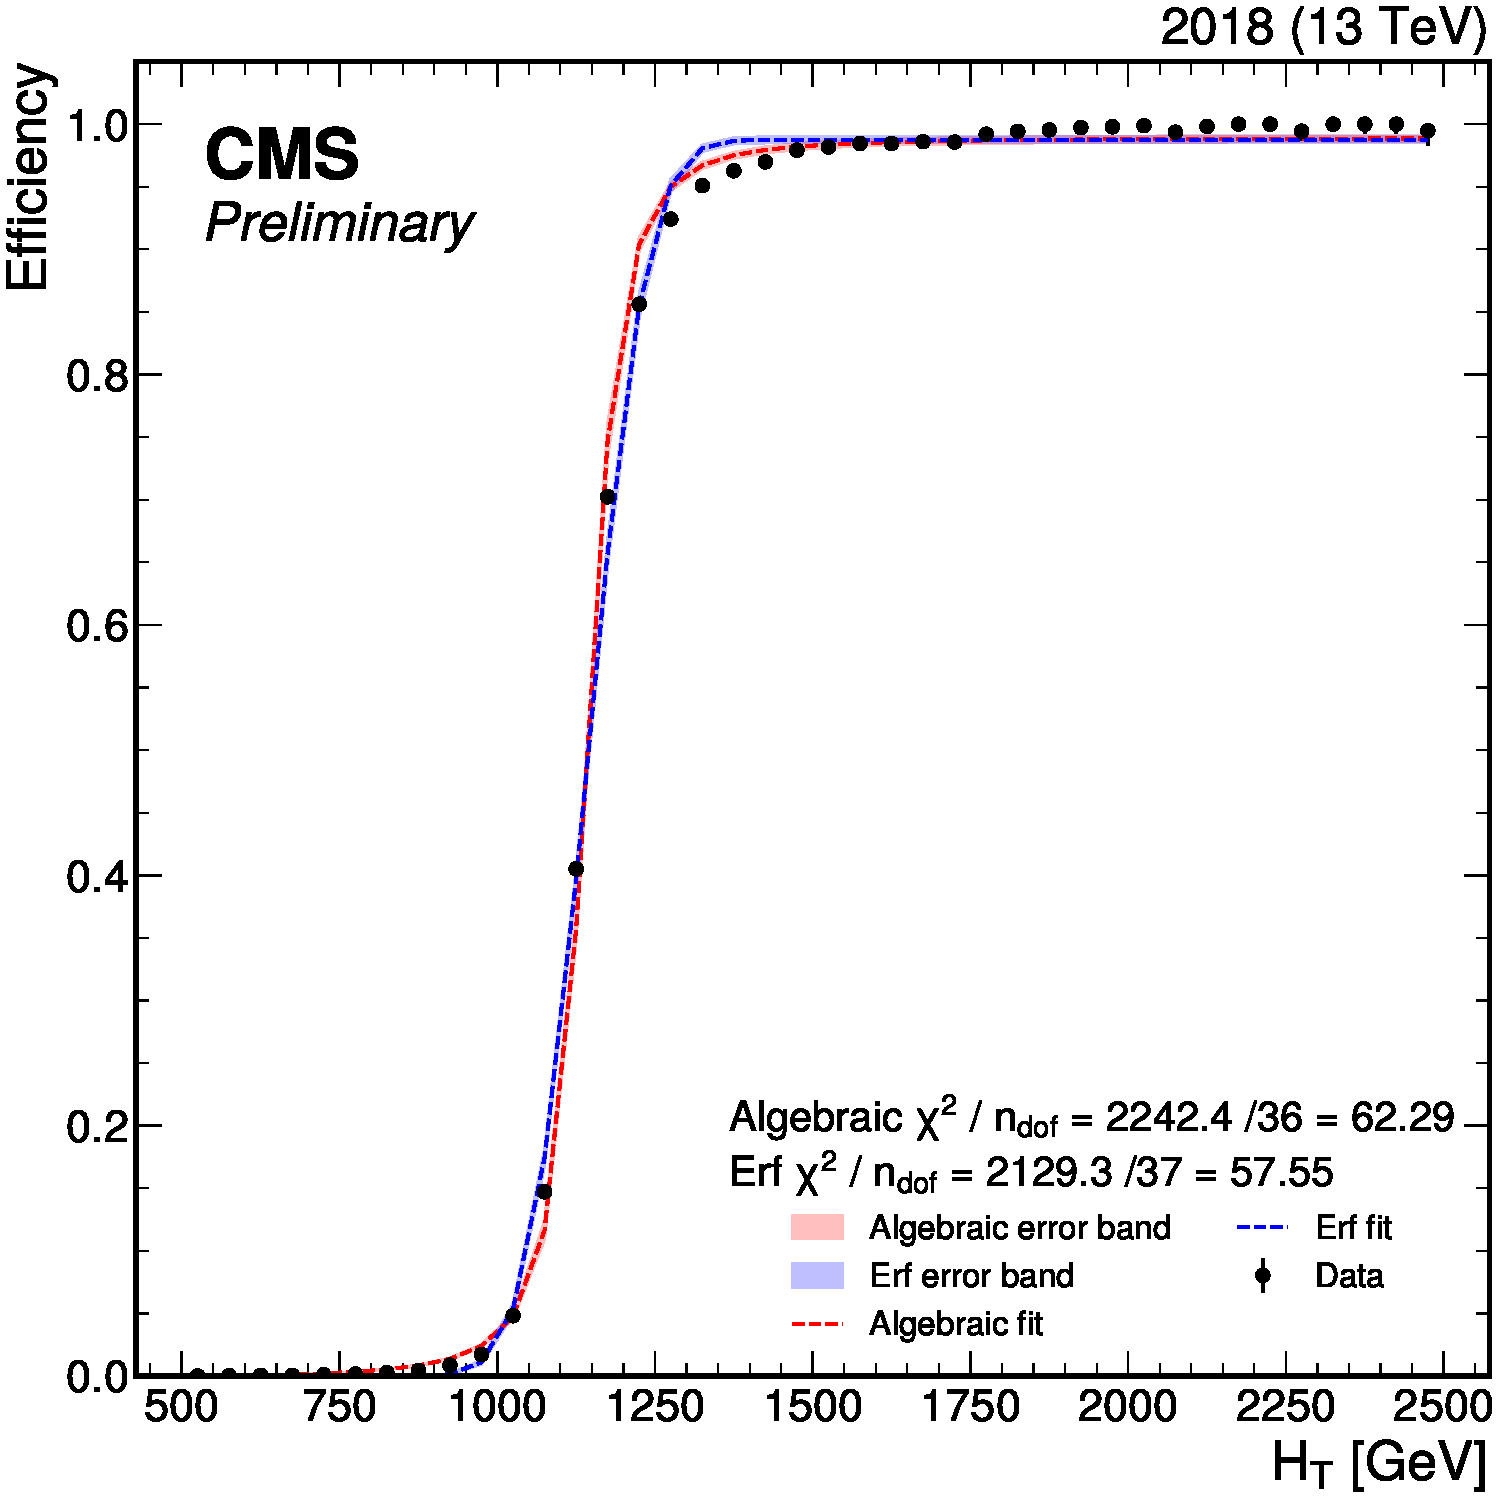
\includegraphics[width=\linewidth]{Images/pdfs/fits_18.pdf}
		% \caption{Caption}
		% \label{fig:enter-label}
	\end{subfigure}%
	\begin{subfigure}{.36\linewidth}
		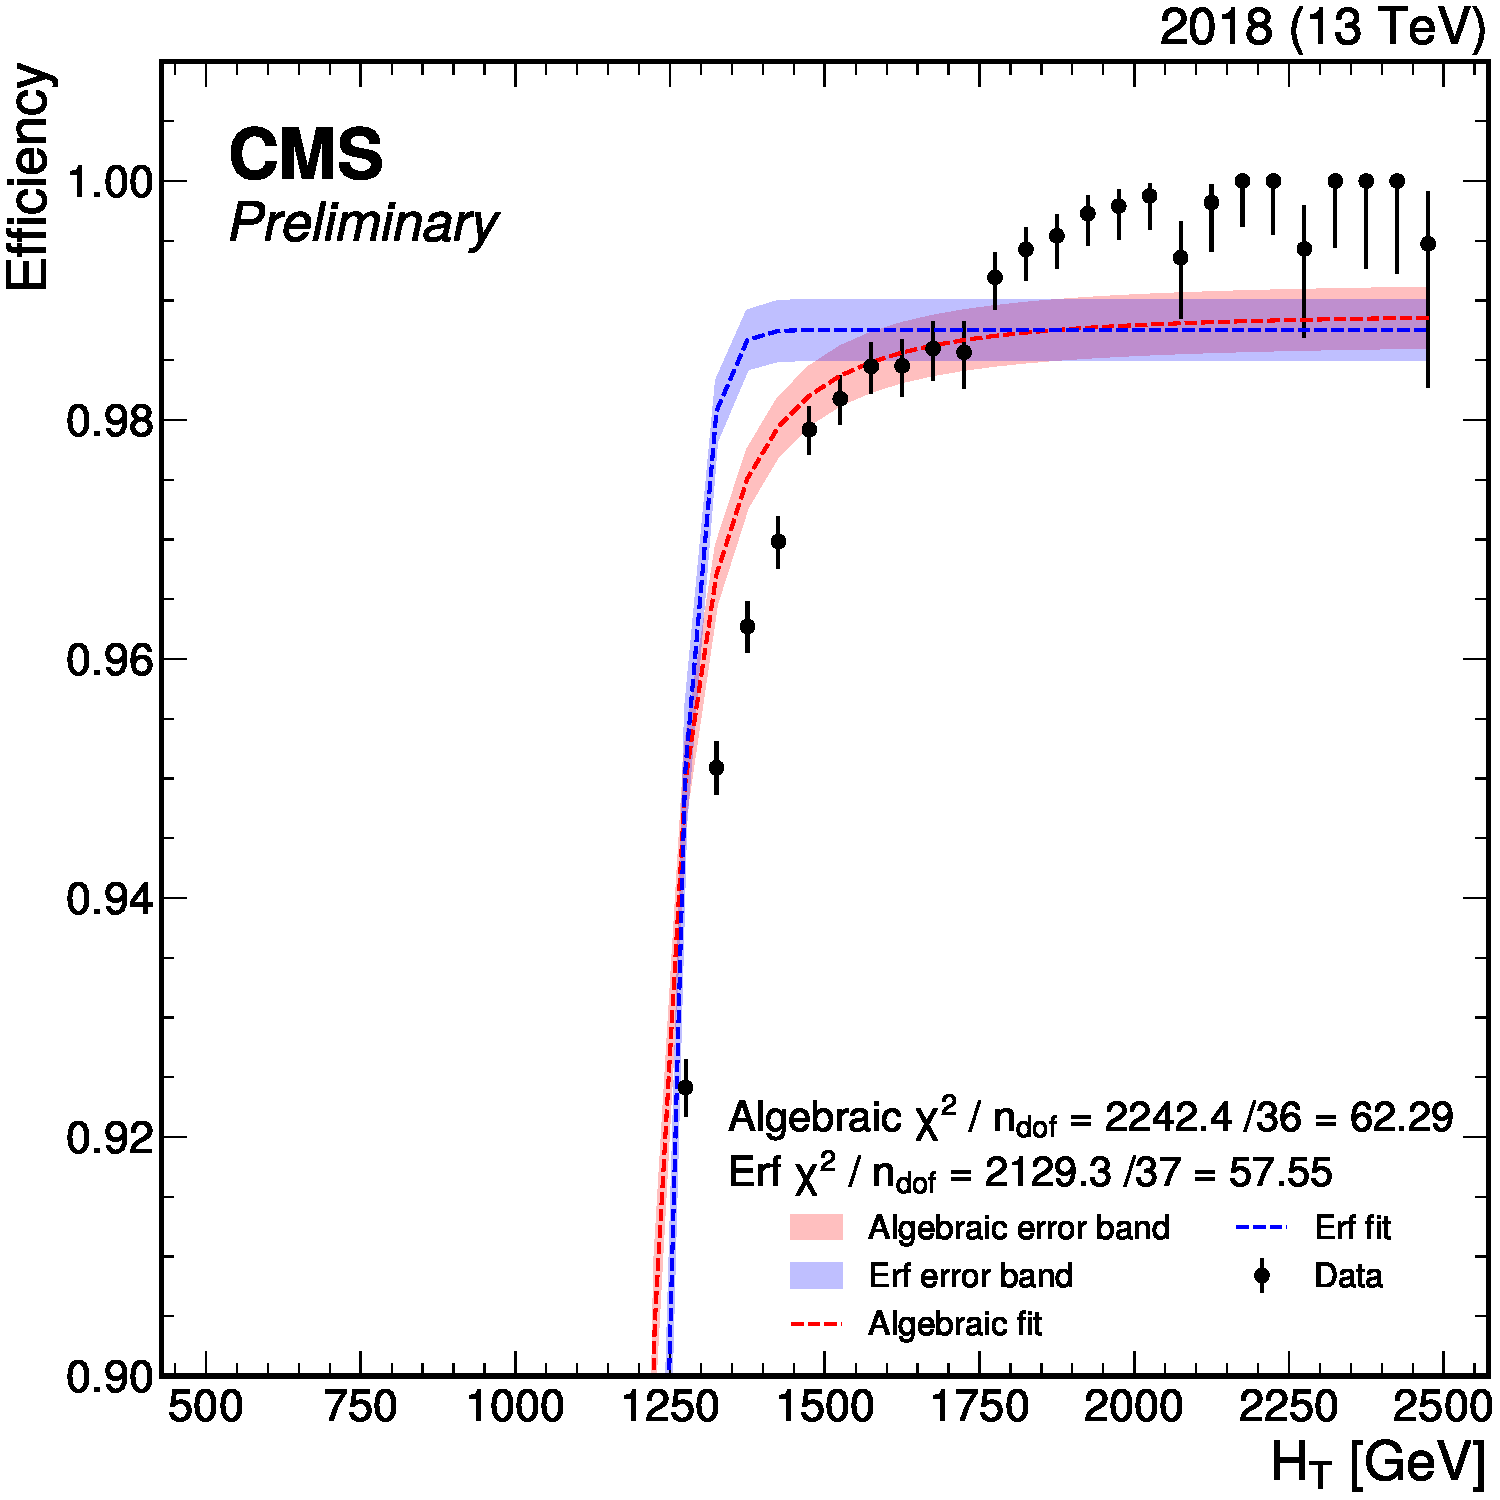
\includegraphics[width=\linewidth]{Images/pdfs/fits_closeup_18.pdf}
		% \caption{Caption}
		% \label{fig:enter-label}
	\end{subfigure}
	\caption{More detailed plots that show information about the goodness-of-fit, namely de $\chi^2$ statistic.}
	\label{fig:fits}
\end{figure}

\clearpage


\chapter{Data Quality Monitoring (DQM) \label{ch:DQM}}
DQM is for a high-quality data where increasing data size (10 times more Pixel readout channels for Inner Tracker alone during HL-LHC) is creating a huge challenge for shifters to monitor and certify it.  Use of ML techniques in DQM can aid shifters detect data anomalies as detector conditions change. Currently, a shifter assesses data quality by a manual scrutiny - comparing histograms with reference ones, looking for any deviations.
We are exploring ML Playground (MLP), a Django-based framework, to automate DQM. It groups training dataset information, automates ML training, and generates reports based on the performance of ML model.
Fidalgo [31] developed a python code to extract information from Run Registry (RR) on Good/Bad runs. RR along with (1) DQM graphical interface (for 1D and 2D histograms), (2) OMS (Online Monitoring System, for beam conditions like luminosity, pile-up, trigger info) and (3) TkMaps (Tracker Maps for information organized geometrically to visualize issues and data trends in detector components) provides input to the ML framework. Fig. 6 shows a cronjob script by Fidalgo to execute DAS queries and copy files to any area with password-less certificate.


There are two future tasks: Task 1 requires upload of newly collected data from DQMIO (Data Quality Monitoring Input Output) to the ML Playground Graphical User Interface (GUI) and organizing it efficiently for ML use. It requires (1) developing scripts to upload DQMIO files to the dedicated EOS space (EOS provides fast and reliable multi-PB disk-only storage) and track the "health" of the files uploaded, (2)  monitor the file system at regular intervals and discover newly uploaded files, (3) run the MLP parser on the new files, (4) implement robust checks of the files already present in the EOS space and attempt to copy over only newly added files to the list and (5) implement a method that allows for files that are already found in the EOS to be forcibly updated or overwritten at the request of a user, if needed and (6) add logging functionality for detailed bookkeeping in case scripts involved fail. This entails use of DAS (Data Aggregation System) query for files in datasets of interest, iterate through the content generated and copy it to EOS where all DQMIO files are stored for the GUI.
Task 2 will develop a Reference Run Ranking (RRR) tool based on the files provided. When a target run (i.e., a run that the shift leader needs to find a reference run for, during Data Certification (DC) and a set of prior candidate runs are provided to RRR, it will rank these candidate runs from best to worst based on their suitability as reference runs. This should ease the reference run selection and, by identifying high-quality runs, serve as a resource for shifters to find robust training datasets for ML models accessible through the MLP. A reference run should meet two criteria: (1) contain a high amount of LumiSections (LS) to ensure statistical robustness and (2) the run’s data-taking conditions should be as similar as possible to those of the target run.
Past efforts failed to consistently place the reference run at the top of the list of candidates due to two main problems: firstly, the parameters characterizing each run were not normalized, leading to an artificial inflation of the importance of some parameters over others and secondly, the weights assigned to each parameter were not systematically determined but were instead based on expert opinion and experience. To mitigate these issues, feature vectors would be constructed for both target and candidate runs using (1) Run level features like initial luminosity, end luminosity, change in luminosity, delivered luminosity, start time of the run, and run number and (2) LS level features like average and standard deviation of initial luminosity, average and standard deviation of the end luminosity, average and standard deviation of pileup. Weighted Euclidean distance between feature vectors of the candidate runs and the target run would be computed to gauge similarity between them. A systematic approach would be implemented to determine the appropriate weights for this metric, that will include the normalization and possible standardization of features to ensure that they are comparable irrespective of the statistical approach chosen.


\chapter{Conclusion}\label{ch:conclusion}

There are three major topics of research that were discussed in this dissertation: The simulation studies involving the counting of L1-stubs for the HL-LHC CMS Inner Tracker upgrade ({stubs}), the overall 2016 search for SUSY in the all-hadronic channel using a customized top-tagger ({AnalysisChap}) and the improvements made for the estimation of the Z$\rightarrow \nu\bar{\nu}$+ jets background using an additional control region from $\gamma$+ jets events ({estimation}). These studies were explained in detail in their respective chapters and their individual results are provided. A summary of the most important results from each study is provided in this chapter.

\section{L1 Stub Counting for the HL-LHC CMS Tracker Upgrade}

Results from this study (detailed in {stubs}) reflect the overall effects that were expected beforehand. The removal of discs from the standard pixel geometry (consisting of 8 small and 4 large discs) results in a noticeable reduction of stub hits in the upgraded CMS Outer Tracker. This effect is specially apparent if the disc that is removed is closer to the interaction point, due to the much larger volume of particles that are present in this region. Therefore, the reduction in stubs is more pronounced when a small disc is removed (as in the case of the $7s4l$ geometry) than if a large disc is removed (as in the $8s3l$ pixel geometry). The reason for this effect stems from the fact that as particles travel through the various layers of the Inner Tracker material, some of them are bound to interact with it, producing particles that did not originate from the initial proton-proton collision. The stubs produced via such processes are considered to be ``fake'' stubs. To confirm these findings, an additional study was conducted using a sample that was virtually indistinguishable from the standard pixel geometry, but with the second disc on the positive side ``turned off'' or ``dead''. The results from this study confirm the initial findings and shows that there is indeed a correlation between the average number of stubs detected in the Outer Tracker and the total amount of material present in the upgraded Inner Tracker. An important factor that needs to be taken into account when interpreting these results is the re-optimization of the disc positions after removing a disc in the different pixel geometries considered. This feature could provide a possible explanation as to why the $6s3l$ geometry, which has two less small discs than the standard geometry (and one less large one), was found to have less of an effect on the average number of stubs than the $7s4l$ geometry.

\section{Search for SUSY in the All-Hadronic Channel}

The analysis presented in {AnalysisChap} shows the results of a search for SUSY in the 0-lepton final state using a customized top-tagger. The data was obtained from proton-proton collisions at the CMS detector during 2016 with a total integrated luminosity of 35.9 fb$^{-1}$ at a center-of-mass energy of 13 TeV. The search was conducted by specifying 84 non-overlapping regions of phase space with varying requirements on the $N_\text{b}$, $N_\text{t}$, $p_{\text{T}}^{miss}$, $H_\text{T}$ and $m_\text{T2}$ variables ({SearchBinDef}). Several dominant and non-dominant backgrounds were identified and estimated to account for all the majority of the processes that were seen in the collected data. The estimation procedures and their respective systematic and statistical uncertainties are discussed in {backgrounds}. The total background prediction vs. data for all 84 search bins ({SearchBinResults}) shows no statistically significant deviation from the predicted SM background. The biggest sources background were shown to be the t$\bar{\text{t}}$ and W+jets processes, followed by Z($\nu\bar{\nu}$)+jets, which were seen to be dominant in regions with a high $p_\text{T}$ threshold. Meanwhile, the contributions from the QCD multijet and rare backgrounds are found to be nearly negligible in all of the 84 search bins. Exclusion limits were calculated from these results for each of the signal models used, by applying a binned likelihood fit on the data. The likelihood function was obtained for each of the 84 search regions as well as for each of the background data control samples from the product of the Poisson probability density function. Exclusion limits were placed on the top squark, gluino and LSP production cross-sections with a 95\% confidence level (CL), calculated using a modified frequentist approach with the CL$_s$ criterion and asymptotic results for the test statistic. The 95\% CL exclusion limits obtained for the T2tt model, which consists of direct top squark production, excludes top squark masses up to 1020 GeV and LSP masses up to 430 GeV. For the T1tttt model, gluino masses of up to 2040 GeV and LSP masses up to 1150 GeV are excluded, with corresponding limits of 2020 and 1150 GeV for the T1ttbb model, 2020 and 1150 GeV for the T5tttt model, and 1810 and 1100 GeV for the T5ttcc model.

% \backmatter


\printbibliography[keyword = content, heading=bibintoc]
\printbibliography[keyword = {th}, heading=subbibintoc,title={Talks related to thesis work given at conferences}]

\appendix

\chapter[Appendix]{\hypertarget{appendix}{}}


Besides the above, I have also contributed to HEP Snowmass process \cite{snowmass_site} in Community Engagement Frontier \cite{snowmass_engagement}. In particular, I co-authored papers in CommF4: Physics Education \cite{snowmass_edu}  and CommF2: Career Pipeline \& Development \cite{snowmass_carrerdev}. This led to three publications \cite{malik2022broadening,bardeen2022particle,malik2022facilitating}.

I have also been an integral part of mentoring in the USCMS internship program~\cite{pursue_site,fnal_int} at Fermilab and have been acknowledged here \cite{bose2022us,banerjee2024novel} where I have co-developed software curriculum for the interns and been an instructor for past three years.

% My work on broader impacts on outreach in HEP has led to the following publications


% \cite{snowmass_site,snowmass_engagement,snowmass_edu,pursue_site,fnal_int}

The software experience gained from this work enabled me to disseminate my experience to students from UPRM and the international HEP community. I have organized several Python and HEP data analysis trainings and workshops, in Puerto Rico at UPRM and HEP worldwide \cite{carp21,carp22,carp22b,DAFLR,matplot,MLatCROEM23,PythoSeriesBasics,PythoSeriesMatplot,PythoSeriesML,PythoSeriesPandas,UPRM_ML_Undergrad}.
This has been an extremely fruitful outcome of my learning experience and a great sense of giving back to the community.


\printbibliography[keyword=page,title={Snowmass and US CMS Internships URLs},heading=subbibintoc]

\printbibliography[keyword=pubs,title={Publications on Broader Impacts},heading=subbibintoc]


\printbibliography[keyword=workshop,title={Software Trainings and Workshops},heading=subbibintoc]






% \cite{CUpathways,UMCERN2018,pyhep22,root-workshop,uprm-fair}


% \chapter{Jargon words}

% \printbibliography[heading=bibintoc]
% list of thesis related talks at conferences or meetings

\end{document}
